\documentclass[12pt,a4paper,openright]{book}
\usepackage{graphicx}
\usepackage[spanish, english]{babel}
\usepackage[utf8]{inputenc}
\usepackage[nottoc]{tocbibind}
\usepackage{appendix}
\usepackage[breaklinks,backref=true,colorlinks=true]{hyperref}
\usepackage{fancyhdr}
\usepackage{comment}
\usepackage{url}
\usepackage{todonotes}
\usepackage{wrapfig}
% \usepackage{layout}

\graphicspath{{figs/}}

% Comandos para consultar la fecha y el título del documento
\newcommand{\thedate}{\today}
% \newcommand{\thetitle}{Electrolites}
\newcommand{\thetitle}{Low-power Wireless ECG Monitoring System for Android Devices}

\setlength{\parindent}{0in}

\title{\thetitle}
\author{Pablo Fernández\\Rafael de la Hoz\\Miguel Márquez}

\hypersetup{backref=true, colorlinks=true, linkcolor=black, menucolor=black,
	urlcolor=black, citecolor=black}

\begin{document}

	% \layout

	%\maketitle
	\frontmatter % Para prólogos y abstracts y cosas así (numeración romana)
	\pagestyle{fancy}

	%\listoftodos
	
	% Redefinición del estilo plain para cambiar los inicios de capítulos
	\fancypagestyle{plain} {
		\fancyhf{}
		\fancyfoot[RO,LE]{\thepage}
		\renewcommand{\headrulewidth}{0.0pt}
		\renewcommand{\footrulewidth}{0.0pt}
	}

	% Sin encabezados ni pie de página, sólo la numeración de la página
	\pagestyle{plain}
	\fancyhf{}
	\fancyfoot[RO,LE]{\thepage}
	\renewcommand{\headrulewidth}{0.0pt}
	\renewcommand{\footrulewidth}{0.0pt}

	% Documentos anteriores al índice
	\thispagestyle{empty}

\begin{center}
	{\Huge \textbf{\thetitle}}

	\vspace{1cm}
	{\large
		Pablo Fernández\\
		Rafael de la Hoz\\
		\vspace{1mm}
		Miguel Márquez
	}

	\vspace{1cm}
	PROYECTO DE SISTEMAS INFORMÁTICOS\\
	FACULTAD DE INFORMÁTICA\\
	Complutense University of Madrid
	\vspace{1cm}

	\includegraphics[scale=.8]{ucm}\\
	\vspace{.5cm}
	Department of Computer Architecture and Automation\\
	\thedate
\end{center}

\begin{flushright}
	Directors:\\
	Luis Piñuel Moreno\\
	Joaquín Recas Piorno\\
\end{flushright}


	\chapter{Abstract}
\label{cha:abstract}

	{\small 
	\paragraph{} People affected by specific cardiovascular diseases require of a constant monitoring of their vital signs, to which end specialized, high priced and big sized equipment is employed. Reduction of the energetic requirements and improvement of the portability are the objectives for the next generation of monitoring systems. This document presents the development of a low-power wireless ECG monitoring system for Android devices. By using the mobile phone or tablet of the user the total amount of needed devices is limited, and the application of the 802.15.4 wireless communication standard substantially decreases the energetic consumption when compared to wider spread ones like Bluetooth. The development of an USB 802.15.4 receiver device and the Android monitoring application results in a system targeting as unintrusive operation as posible. Systems such as this one have proved to be highly useful and a generalization of their employment is to be expected.
	\paragraph{Keywords}	
	ECG, Android, MSP430, FreeRTOS, Shimmer, USB, 802.15.4
	}\\
	
	{\small 
	\paragraph{} Las personas afectadas por ciertas enfermedades cardiovasculares requieren de una estrecha vigilancia de sus constantes vitales, lo cual supone el empleo de equipos especializados de elevado coste y tamaño. La reducción del consumo energético y el aumento de la portabilidad son los objetivos de la próxima generación de dispositivos de monitorización. En este documento se presenta el desarrollo de un sistema inalámbrico de monitorización electrocardiográfica portátil de bajo consumo para dispositivos Android. Al reutilizar el terminal del usuario se reduce el número de dispositivos necesarios, y la aplicación del estándar de comunicación inalámbrica 802.15.4 disminuye el consumo de energía de forma significativa respecto al uso de otras alternativas como Bluetooth, la más empleada en este ámbito. El desarrollo de un receptor USB 802.15.4 junto con la aplicación de monitorización para Android resulta en un sistema orientado a ser lo menos invasivo posible en la vida del usuario final. Sistemas de estas características han desmostrado ser de gran utilidad y se espera un uso generalizado de los mismos en casos de necesidad de monitorización constante.
	\paragraph{Palabras clave}
	ECG, Android, MSP430, FreeRTOS, Shimmer, USB, 802.15.4
	}



\newpage % disclaimer
	\paragraph{}
	Pablo Fernández, Rafael de la Hoz and Miguel Márquez authorize Complutense University 
	of Madrid to spread and use this report and the associated code, multimedia content and its results with academical and non-comercial purposes,
	provided that its authors shall be explicitly mentioned.
	\begin{center}
    	\thedate \\
	    \vspace{5.5in}
		Pablo Fernández\hspace{0.75in}
		Rafael de la Hoz\hspace{0.75in}
		Miguel Márquez
	\end{center}

	\chapter*{Acknowledgements}
\label{sec:acknowledgements}
	
	% Los agradecimientos que vayamos a hacer
	

	\tableofcontents % Índice

	% Para la lista de figuras y la de tablas, lo mismo
	\pagestyle{plain}
	\fancyhf{}
	\fancyfoot[RO,LE]{\thepage}
	\renewcommand{\headrulewidth}{0.0pt}
	\renewcommand{\footrulewidth}{0.0pt}
	\listoffigures
	\listoftables

	\chapter{Resumen en español}
\label{ch:resumen}
	\selectlanguage{spanish}
	% Descripción del proyecto
	En este proyecto se expone la investigación realizada con el objetivo de desarrollar un receptor del estándar de redes de área personal inalámbricas 802.15.4 del IEEE para dispositivos Android a través de USB, aplicado a un sistema completo de monitorización electrocardiográfica (ECG), así como el proceso de desarollo del mismo. Este sistema se enmarca en el ámbito de la atención sanitaria personal: su principal aplicación es la montorización del estado del corazón por parte de un particular, eliminando la dependencia, respecto a esta tarea específica, con los sistemas de atención sanitaria tradicionales.\\

	Recientemente ha surgido un gran interés, tanto en el ámbito académico como en el industrial, en la producción de sistemas de monitorización ECG portátiles y de bajo consumo, llegando a ser una de las principales aplicaciones de las redes de sensores corporales inalámbricas.\\

	Para maximizar la portabilidad, en el desarrollo de estos sistemas se han empezado a emplear dispositivos móviles de gran capacidad de cómputo, particularmente smartphones, debido a la gran difusion que han tenido en los últimos años. En el 2011  se presentó un sistema, colaboración entre la Universidad Complutense de Madrid (UCM) y la École Polytechnique Fédérale de Lausanne (EPFL), para monitorización ECG de ámbito personal empleando un iPhone como visualizador y Bluetooth como tecnología de comunicación inalámbrica\todo{Citas en el resumen?}.\\

	De los resultados obtenidos por ese proyecto surge la presente iniciativa que trata de llevar al siguiente nivel las características inherentemente buenas de bajo consumo y bajo coste del mismo mediante la aplicación del protocolo 802.15.4, de mucho menor consumo energético que la tecnología Bluetooth, y la sustitución del dispositivo iOS por uno basado en Android, debido a su mayor accesibilidad y el menor coste, en general, de éstos.\\

	El sistema desarrollado en este proyecto presenta al usuario una representación visual de su onda ECG en tiempo real, resaltando puntos relevantes para simplificar la compresión de los datos mostrados. También muestra información sobre el ritmo cardiaco, y toda esta información es almacenada de forma transparente al usuario para su posterior consulta.\\

	Esta funcionalidad es posible gracias a la operación conjunta de los tres dispositivos que forman el sistema de monitorización: el nodo de delineación ECG, el receptor 802.15.4 y el dipositivo Android que actúa de interfaz con el sistema. El nodo de delineación ECG va conectado a la red de sensores corporal del usuario y se encarga de la captura y posterior análisis de la onda ECG, así como de la codificación y envío de la misma de forma inalámbrica. El receptor 802.15.4 conectado al sistema Android a través de USB controla la recepción de datos a traves de dicho protocolo y el envío de la información recibida al dispositivo Android. Éste actúa como decodificador y visualizador en tiempo real, y, como interfaz con el sistema, gestiona las conexiones inalámbricas y almacena y muestra los datos recibidos.\\

	Los objetivos del proyecto son, entonces, el desarrollo de la aplicación para dispositivos Android, la producción del receptor 802.15.4 y la comunicación de ambos con un nodo delineador ECG ya existente.\\

	La aplicación para dispositivos Android, como ya se ha mencionado, es la interfaz con la que el usuario interactúa con el sistema. Su diseño sigue las prácticas comunes de aplicaciones para este sistema operativo ya que el objetivo es que la curva de aprendizaje sea, si no nula, muy suave. Los motivos para emplear Android como sistema operativo base son tres: la importancia de éste entre los sistemas operativos móviles, el mayor rango de precios de los terminales que lo soportan, que permite una mayor difusión del sistema debido a la existencia de dispositivos de precio más reducido, y la naturaleza libre y de código abierto del entorno de desarrollo, característica que facilita la posterior expansión del sistema. Todos estos motivos pueden resumirse en que el empleo de Android como sistema operativo permite el acceso de un mayor número de usuarios al mismo.\\

	En cuanto al nodo delineador de la onda ECG, el objetivo es emplear uno ya desarrollado para el proyecto. Esto es así porque tanto el nodo delineador como la red de sensores corporales que capturan la onda ECG son sistemas especialmente complejos cuyos desarrollos ocuparían, cada uno, un proyecto de la envergadura del actual.\\

	El nodo delineador que se emplea en el proyecto es obtenido en el proyecto de la UCM y la EPFL antes mencionado. Este nodo se desarrolló inicialmente como un delineador de electrocardiografía en tiempo real de bajo consumo con capacidad para envíar los datos de forma inalámbrica a través de Bluetooth. En otro esfuerzo conjunto entre la EPFL y la UCM se dotó al nodo de funcionalidad para el envío empleando 802.15.4, pero tan sólo al nivel necesario para realizar algunas estimaciones de consumo. Incluso con la utilización real del estándar 802.15.4 estando aún por llegar, el nodo presenta las características necesarias para convertirse en un excelente punto de partida para el alcance de los objetivos del proyecto.\\

	El componente más importante del sistema en cuanto a este proyecto se refiere es el receptor USB de 802.15.4 en tiempo real para dispositivos Android. Su desarrollo es una necesidad puesto que los dispositivos Android actualmente no proporcionan soporte para el protocolo 802.15.4, aunque sí para otros como Bluetooth o Wi-Fi. Considerando que en el nodo delineador que se toma como punto de partida para el sistema la operación que supone mayor consumo de batería es la utilización de la infraestructura Bluetooth, como confirman los estudios realizados por la UCM y la EPFL, la producción del receptor 802.15.4 es, pues, imperativa.\\

	La existencia de otros proyectos con el objetivo de la dotación a dispositivos móviles del estándar 802.15.4 es un hecho conocido desde el inicio del proyecto, aunque éstos no tengan como objetivo el campo de la biomedicina o la monitorización personal. El motivo para no apoyar o emplear alguno de ellos es doble: por un lado, al comienzo del proyecto éstas iniciativas se encuentran o bien inconclusas o bien paralizadas; más aún, todas son proyectos aislados, generalmente desarrollados por una única persona y sin ningún tipo de soporte oficial ni garantías de finalización. Por otra parte, y siguiendo la idea de obtención de un sistema de tamaño reducido, el objetivo de este proyecto es emplear el dispositivo Android como maestro en la comunicación USB, de forma que el receptor 802.15.4 obtenga la alimentación a través de él, eliminando así la necesidad de emplear una batería que incrementaría el tamaño del receptor. Ninguno de los proyectos existentes emplea la capacidad de los dispositivos Android para asumir el rol de maestro en la comunicación, así que no son de utilidad real para el proyecto.\\

	% Motivación
	El desarrollo del proyecto viene motivado por dos razones principales: la 
	potencial utilidad que demuestra tener un sistema de estas características 
	y el interés que suscita a nivel académico.\\

	Según la Organización Mundial de la Salud (OMS), las enfermedades cardiovasculares representan la
	principal causa de mortalidad a nivel mundial. Sin embargo, la vigilancia que requieren las
	personas afectadas no es asumible, por lo general, por los sistemas de sanidad tradicionales. La
	monitorización doméstica continua supondría una gran ayuda para estas personas, pero todavía
	se trata un objetivo a cumplir.\\

	En un escenario como este, las redes inalámbricas de sensores corporales (wireless body sensor
	networks, WBSN) se presentan como herramientas de monitorización eficientes y asumibles
	económicamente. Particularmente, las WBSN aplicadas a la monitorización electrocardiográfica son
	de gran utilidad en el seguimiento de enfermedades cardiovasculares. De hecho, proyectos como el
	de la UCM y la EPFL mecionado anteriormente promueven la expansión de sistemas como estos.\\

	Además, con el uso de dispositivos portátiles, en particular smartphones, para mostrar los
	resultados de la monitorización se persigue la expansión de estos sistemas en todos los ámbitos
	de la sociedad, ya que permiten integrar el sistema en dispositivos ampliamente utilizados, 
	evitando así la necesidad de cargar con aparatos adicionales. La elección de Android como 
	plataforma reponde a	los factores de difusión y menor coste de los terminales que se mencionaron 
	anteriormente, con el objetivo principal 	de maximizar la expansión del sistema.\\

	Asimismo se busca el uso más extendido del sistema con el aumento de la duración de la
	batería y la reducción del tamaño de los nodos de monitorización: un consumo de batería menos
	exigente permite un número menor de interrupciones en la monitorización producidas durante el
	proceso de carga de la misma, mientras que el menor tamaño del dispositivo facilita el emleo
	contínuo del mismo. La utilización del estándar 802.15.4 responde a la búsqueda de la
	realización de estos objetivos.\\

	En conjunto, el uso de un dispositivo Android con capacidad de recepción 802.15.4 en un
	sistema de monitorización electrocardiográfica continua rebaja los requisitos de consumo de batería
	y tamaño del sistema completo, y de esta forma mejora la posibilidad de ser transportado y relaja
	las restricciones en su aplicación.\\

	Desde un punto de vista académico, la principal motivación que plantea el desarrollo de este
	proyecto es el hecho de que reune prácticamente todas las áreas de la carrera de Ingeniería
	Informática. Desde el mismo comienzo el proyecto implica desarrollo tanto software como
	hardware además de investigación en ámbitos externos al alcance de la propia carrera,
	como tecnologías inalámbricas de bajo consumo	o desarrollo para dispositivos móviles, así como 
	tareas de diseño y desarrollo en un amplio rango de niveles de abstracción.\\

	Se espera también que las tecnologías basadas en la especificación del estándar 802.15.4 del IEEE
	como ZigBee verán incrementada su relevancia a medio plazo debido a sus potenciales aplicaciones en
	campos como la domótica y la biomedicina, entre otros.\\

	Además, tanto el desarrollo de aplicaciones como de accesorios para smartphones u otro tipo de
	dispositivos portátiles son unas de las prácticas más habituales hoy en día en el ámbito del
	desarrollo de sistemas informáticos, y representan algunas de las actividades más demandadas. Por
	tanto, entrar en contacto con ellas proporciona una experiencia adicional en un campo puntero que
	no hace sino amplíar nuestro rango de habilidades y, por consiguiente, incrementa nuestro valor en 
	el mercado laboral.\\

	% Desarrollo
	Al comienzo del proyecto, evaluando los objetivos, se decide hacer una distinción muy clara entre dos partes del proyecto: por un lado, el desarrollo de la aplicación para Android y por otro, la investigación orientada al posterior desarrollo del receptor 802.15.4 así como la correcta utilización del nodo delineador seleccionado incluyendo las modificaciones que hubiera que hacerle al mismo.\\

	El desarrollo la aplicación Android se trata de un proyecto de desarrollo software de tamaño manejable cuyo mayor riesgo consiste en la falta de formación del equipo en el ámbito del desarrollo de aplicaciones para dispositivos móviles.\\

	Por su parte, el desarrollo del receptor 802.15.4 implica un esfuerzo de investigación hardware importante, ya que la mayoría de los objetivos planteados ni siquiera se sabe si son alcanzables. Es más, el desarrollo de dispositivos electrónicos al nivel requerido por el proyecto queda fuera del alcance de la formación recibida. Todo esto provee a la parte de desarrollo e investigación sobre hardware de un nivel de incertidumbre, tanto en la posibilidad real de alcanzar los objetivos propuestos, como en la capacidad del equipo para llevarlos a cabo, muy superior al existente en el desarrollo software.\\

	Esta situación propicia la división del proyecto en dos subproyectos a desarrollar de forma independiente pero teniendo en cuenta en todo momento la estrecha relación entre uno y otro. De esta forma en cada desarrollo se pueden aplicar las metodologías, técnicas y planificaciones más apropiadas para el tipo de trabajo concreto a realizar. Atendiendo a la estrecha dependencia entre los dos proyectos, y buscando evitar grandes descompensaciones entre ambos, se fija una planificación común a todo el proyecto de forma que ciertos hitos deben alcanzarse a la par en ambos desarrollos.\\

	De esta forma se asegura que la funcionalidad producida por un proyecto se completa en el otro mientras se deja libertad para aplicar el enfoque que se considere más efectivo en cada proyecto durante los ciclos de desarrollo. Además, dada la incertidumbre asociada a la investigación hardware, los plazos temporales para los hitos se asumen como variables y se manejan planes de actuación en la planificación del proyecto de desarrollo software para que el trabajo no se vea detenido por los potenciales retrasos. Se considera, entonces, que el camino crítico del proyecto está definido por el proyecto de investigación y desarrollo hardware y el proyecto de desarrollo software debe adaptarse a sus necesidades. Aún y así en la planificación del primero no se dejan de tener en cuenta las posibles contingencias del desarrollo software.\\

	La tecnología seleccionada para el desarrollo del proyecto es la siguiente:
		\begin{itemize}
			\item \emph{El dispositivo móvil tipo tableta basado en Android} Motorola Xoom
			
			Escogido entre otros modelos de terminales que soportan Android por su capacidad para asumir el rol de maestro en la comunicación USB. Además, la capacidad del procesador que incorpora y el hecho de integrar una GPU lo hacen especialmente aplicable para la consecución del objetivo de mostrar los datos de la electrocardiografía en tiempo real.
		
			\item \emph{Nodo delineador de ECG producido por la UCM y la EPFL}

			Este nodo se basa en la plataforma inalámbrica de sensores corporales \emph{Shimmer} para la captura de la onda electrocardiográfica y realiza un análisis de la misma (denominado delineación), enviando los datos a través de Bluetooth o, potencialmente, 802.15.4. El nodo se encuentra completamente desarrollado y validado al comienzo del presente proyecto, salvo la funcionalidad de envío a través de 802.15.4, que si bien está implementada en el dispositivo, no se ha probado de forma exhaustiva.

			\item \emph{La familia de microprocesadores de 16 bits} MSP430 \emph{de la firma} Texas Instruments

			Su elección se realiza teniendo en cuenta tanto su reducido consumo de energía como la sencillez en su programación, que permite utilizar C y depurar a través del estándar JTAG; pero principalmente por el hecho de que el nodo delineador ECG a emplear en el sistema utiliza esta misma familia de microprocesadores, y existe la posibilidad de reutilizar parte del código, especialmente el sistema operativo y la funcionalidad relacionada con envío inalámbrico a través de 802.15.4.\\

			\item \emph{Sistema operativo de tiempo real} FreeRTOS \emph{para dispositivos empotrados}

			El empleo de este sistema operativo viene determinado por la elección del nodo delineador, ya que éste emplea \emph{FreeRTOS} y la implementación de la capa MAC 802.15.4 para dicho sistema operativo se encuentra disponible y puede ser aplicada en el proyecto. Es más, dado que el microprocesador que llevará el receptor a desarrollar es el mismo que el del nodo delineador, el sistema operativo puede ser utilizado directamente en el receptor sin esperar la necesidad de muchas modificaciones. Como se menciona antes, la implementación de la capa MAC 802.15.4 para \emph{FreeRTOS} implementación no está totalmente completa, pero es un buen punto de partida.

		\end{itemize}

	Cada tecnología se aplica en uno de los subsistemas que forman el sistema completo. Aunque se ha trabajado también con otras tecnologías, éstas se irán mencionando a lo largo de la exposición del desarrollo del proyecto que se realiza a continuación, y por tanto se omite su enumeración en este punto. Se analiza primero el desarrollo relacionado con la parte de hardware del proyecto.\\

	El subproyecto de hardware contempla dos fases: por un lado la investigación sobre la factibilidad y la forma de alcanzar los objetivos propuestos, y por otro el desarrollo necesario para alcanzar dichos objetivos. Los objetivos concretos de este subproyecto son:

		\begin{enumerate}
			% \item La realización de un prototipo de comunicación USB con Android empleando una placa de prototipado Arduino
			\item Lograr la comunicación de un microprocesador MSP430 mediante USB con el dispositivo Android
			\item Inclusión de capacidad de comunicación a través USB en FreeRTOS
			\item Empleo de 802.15.4 en FreeRTOS en el procesador MSP430 seleccionado
			\item Asegurar la correcta operación de los módulos USB y 802.15.4 sobre FreeRTOS
			\item Diseñar el circuito impreso específico para dispositivo receptor USB 802.15.4
			\item Validación y producción del dispositivo receptor a partir del diseño
		\end{enumerate}

	Debido a las restricciones de tiempo y de disponibilidad del equipo al tener que hacer frente a este subproyecto en paralelo con el desarrollo software, se toma la decisión de establecer estos objetivos como los hitos para la planificación, añadiendo uno extra que contempla una fase de  prototipado inicial sobre una placa Arduino, que es bastante más sencillo que trabajar directamente con un MSP430 y sirve como toma de contacto inicial. Como se menciona anteriormente, los plazos para estos hitos se establecen tentativamente debido a la incertidumbre de cada objetivo.\\

	Cabe mencionar que en lugar de separar las fases de investigación y desarrollo asociadas a cada objetivo se opta por no establecer límites fijos entre ellas, de forma que cada objetivo comienza con el planteamiento de las potenciales líneas de investigación del mismo. Seguidamente comienza el desarrollo de una de las líneas de investigación propuestas, y si se llega a un resultado negativo, se descarta el trabajo y se selecciona otra línea de investigación. Este sistema, cercano a las metodologías de desarrollo extremas basadas en prototipos, junto con la flexibilidad de la planificación propuesta ha resultado ser clave para la correcta consecución de los objetivos del subproyecto de hardware.\\

	Detallamos ahora el proceso de desarrollo del subproyecto de software. Siendo este más cercano a un desarrollo tradicional, con menos incertidumbre en cuanto al resultado, se opta por aplicar una metodología de desarrollo ordenada con la que se asegure el cumplimiento de los plazos establecidos por el subproyecto de hardware. Debido a que se aplican las mismas restricciones temporales y de compartición de recursos que las expuestas anteriormente para el subproyecto de hardware, precisamente por la conducción de ambos en paralelo, se descarta la aplicación de metodologías de desarrollo con gran dependencia de la producción de artefactos, así como de metodologías que requieran planificaciones fijas.\\

	Se opta, entonces, por la aplicación de una metodología híbrida entre una metodología iterativa y una metodología de desarrollo rápido. Esto se traduce en el establecimiento de una planificación inicial en base a los objetivos del subproyecto de hardware. Esta planificación empareja los hitos del desarrollo hardware con la funcionalidad correspondiente de la aplicación Android y, centrándose en construir la mayor cantidad de funcionalidad posible cuanto antes, distribuye el resto de objetivos del subproyecto software. Además es necesario asumir en todo momento la posibilidad de una modificación en las fechas. \\

	Para hacer frente a ese tipo de contingencias se decide aplicar técnicas propias de metodologías iterativas como el análisis de riesgos y el desarrollo basado en casos de uso. De esta forma se mantiene el foco en el desarrollo de la funcionalidad clave aún cuando sea necesario un reajuste de los plazos o una mayor dedicación de recursos al subproyecto de hardware.\\

	Los casos de uso identificados para el sistema son los siguientes:

	\begin{itemize}
		\item UC1. Visualizar datos obtenidos por Bluetooth
		\item UC2. Visualizar datos obtenidos por receptor USB
		\item UC3. Visualizar datos de un archivo de log
		\item UC4. Ajustar parámetros de visualización
	\end{itemize}

	Como el receptor USB 802.15.4 es la culminación de la investigación hardware, la planificación de los esfuerzos de desarrollo se plantea de forma que todo el resto de la funcionalidad se construya y valide mientras el subproyecto de hardware desarrolla un prototipo del receptor, y una vez se tenga este prototipo se proceda a la implementación de la funcionalidad relacionada mientras se desarrolla la versión final. Gracias a este tipo de planificación y al minucioso análisis de riesgos llevado a cabo durante todo el desarrollo, los objetivos del subproyecto de software también han sido alcanzados de forma satisfactoria.\\

	Se ha logrado, entonces, la producción de un sistema de monitorización electrocardiográfica en tiempo real de bajo consumo y tamaño reducido empleando un dispositivo Android como interfaz con el usuario y el estándar 802.15.4 como protocolo de transmisión de datos inalámbrico. Este sistema provee toda la funcionalidad requerida: visualización de la onda ECG en tiempo real proveniente de nodos tanto 802.15.4 como Bluetooth, almacenamiento de ésta de forma permanente en archivos y su posterior visualización, así como capacidad para configurar los parámetros de la visualización tanto en tiempo real como de archivos. El sistema es, pues, una versión más accesible gracias al empleo de dispositivos Android y con un consumo energético dos órdenes de magnitud menor del sistema producido en 2011 por la Universidad Complutense de Madrid y la École Polytechnique Fédérale de Lausanne, lo cual es el principal objetivo del proyecto.\\

	Este hito se alcanza gracias a la correcta finalización tanto del subproyecto de investigación hardware como del de desarrollo software en que se dividide el proyecto. Las diferencias en el enfoque requeridas por cada subproyecto sumadas a la estricta dependencia entre ambos resultaban una complicación añadida en la previsión del resultado de los dos desarrollos; pero, gracias a la aplicación de planificaciones flexibles pero de objetivos firmes en cada uno que no dejaban de tener en cuenta posibles complicaciones en el otro, y que contaban con planes tanto de contingencia como de actuación ante ellas, se manejaron correctamente ambos proyectos, dando lugar al actual estado de finalización satisfactoria del proyecto.\\

	En cuanto al subproyecto de hardware, la producción del receptor USB de 802.15.4 para dispositivos Android se ha llevado a cabo con éxito. El dispositivo ha evolucionado desde las primeras etapas donde se empleaba una placa de prototipado hasta llegar a ser un circuito integrado diseñado expresamente para el proyecto. Este circuito integrado está completamente diseñado y validado, si bien no ha sido aún producido debido a los costes que ello supondría\todo{Eliminar esto si se hace o whatever}. En su lugar se ha utilizado un prototipo, de tamaño algo más reducido pero construido a partir del diseño final de la placa, para la validación del sistema.\\

	Las dimensiones del prototipo son 7.25 x 6.35 x 3.5 cm y necesita 3.3V de alimentación, aunque es utilizable a partir de 3.0V. La conexión USB es la que proporciona esta alimentación y además permite emplear el dispositivo en cualquier sistema capaz de comunicarse mediante HID, y ha sido probado con éxito tanto en dispositivos Android como en ordenadores ejecutando varias versiones de Windows.\\

	Con respecto a la aplicación para terminales Android producida en el subproyecto de software, proporciona toda la funcionalidad que entra dentro de los objetivos del proyecto de forma robusta y con un diseño similar al de las aplicaciones canónicas de Android. Es una aplicación, dentro del dominio específico de la monitorización electrocardigráfica, con funcionalidad de propósito general, que requeriría cierta especialización para ser realmente útil. Esta especialización deberá añadir funcionalidad para el escenario de aplicación particular, y el análisis de esos escenarios o la posible implementación de alguno de ellos queda fuera de los objetivos del proyecto.\\

	En cualquier caso, siendo conscientes de la necesidad de especialización futura de la aplicación, durante el diseño y desarrollo de la misma se puso un gran énfasis en que, además de ofrecer la funcionalidad requerida, proporcionase un conjunto de herramientas tal que pudiera actuar como un framework sobre el cual se pueda realizar el desarrollo de aplicaciones de monitorización ECG más específicas. Como detalle, mencionar que además de que el sistema está preparado para la inclusión sencilla de nuevas fuentes de datos además de Bluetooth, 802.15.4 y archivos, la fuente de datos de 802.15.4 en realidad es un dispositivo USB, en concreto el receptor, por lo que podría emplearse cualquier otro periférico que enviase datos con la codificación esperada en su lugar.\\

	Esto da una idea de la flexibilidad buscada, y alcanzada, del sistema de monitorización desarrollado. Apoyándose en ella, se plantean potenciales líneas de trabajo futuro, distinguiendo entre las que se podrían realizar a corto plazo y las que serían ya para un medio o largo plazo.\\

	Por un lado, un particular afectado de una enfermedad cardiovascular que requiere de monitorización electrocardiográfica constante, observando los objetivos y los resultados del proyecto actual, presentó al departamento un proyecto de especialización del sistema desarrollado para sus necesidades particulares, que son comunes al colectivo de afectados por dicha enfermedad. Este nuevo sistema ha de incorporar, además de la funcionalidad presente en el actual, algunas características nuevas:

	\begin{itemize}
		\item Etiquetado de eventos durante la delineación, de forma que el usuario pueda indicar al sistema en qué momentos se encuentra mal y la información quede almacenada junto a la onda ECG. De esta forma podría estudiarse posteriormente la información guardada de forma más detallada para mejorar la compresión del estado del paciente.
		\item Adición de información temporal a los logs, de manera que el usuario pueda consultar
			directamente la onda ECG relativa a un momento concreto en el que se encontró mal, o que
			pueda saltar al momento indicado por un marcador de eventos. Esto facilitaría la consulta
			y navegación por los datos almacenados.
		\item Comandos de voz que permitan interactuar con el sistema sin necesidad de emplear las
			manos, ya que, ya sea por su estado de salud o porque las tenga ocupadas, es posible que
			el usuario no pueda manejar la aplicación.
		\item Avisos automáticos en caso de que se produzca algún evento relevante relacionado con la
			salud del usuario, de manera que se pueda alertar al mismo, algún pariente o personal
			cualificado en caso de ser necesario. Además, estos avisos podrían hacerse de varias
			formas, ya sea a través de mensaje, correos electrónicos con localización GPS adjunta o
			incluso llamadas de voz automáticas directamente.
	\end{itemize}

	Por otra parte, se contemplan una serie de expansiones del sistema más a largo plazo, debido sobre
	todo a que requieren de más tiempo y recursos, aparte de una planificación específica. En primer
	lugar se proponen mejoras enfocadas a la monitorización de varios pacientes, para un entorno más
	profesional, en dos posibles versiones:

	\begin{itemize}
		\item Dado que el receptor desarrollado también es compatible con dispositivos que soporten el
			protocolo HID, se propone utilizarlo conectado a un PC que actúe como servidor, recibiendo
			los datos ECG procedentes de los nodos de varios pacientes. Una vez estos datos están en
			el servidor, la propia aplicación Android permitiría conectarse a este para descargarlos
			y visualizarlos en el dispositivo.
		\item Teniendo en cuenta que la pantalla de un tablet es relativamente grande, se puede
			aprovechar para mostrar los resultados de la monitorización de varios pacientes a la vez.
			Como parte de esta nueva funcionalidad también se encontraría la de cambiar entre la onda
			ECG de otros pacientes, guardado de logs simultáneo y subida a un servidor dedicado.
	\end{itemize}

	También a largo plazo, aunque en el campo de la automonitorización, se plantea la adaptación del
	sistema a dominios particulares que imponen requisitos adicionales debido, sobre todo, al entorno
	en el que se utilizaría. En este sentido, el director del Laboratorio de Sistemas Empotrados (ESL)
	de la EPFL (equipo responsable junto a la UCM del desarrollo del nodo delineador que se usa en
	este proyecto) ha mostrado interés en la aplicación de los bajos requisitos de consumo del sistema
	en otro proyecto de la EPFL con el que está colaborando, el Solar Impulse.\\

	Este proyecto en concreto trata de conseguir un vuelo alrededor del mundo evitando el uso de
	carburantes de cualquier tipo, utilizando únicamente energía solar. El avión utilizado es de una
	única plaza, por lo que las constantes vitales del piloto deben estar monitorizadas en todo
	momento. Por el momento, la monitorización electrocardiográfica se lleva a cabo utilizando el
	sistema desarrollado por la UCM y la EPFL, con la escasa duración de batería que ello implica.\\

	Teniendo en cuenta que el espacio dentro de la cabina es muy reducido, cualquier tarea debe ser
	llevada a cabo con especial cuidado y únicamente cuando sea absolutamente necesario. Es por ello
	que el intercambio de la batería del nodo delineador debe ser una tarea lo menos frecuente posible,
	entre otras razones porque interrumpe la monitorización en el proceso.\\

	Por tanto, la reducción del consumo de energía y el consiguiente aumento de la duración de la
	batería plantean un avance muy significativo para un proyecto como el del Solar Impulse, tarea
	que se puede conseguir mediante el empleo del estándar 802.15.4 como protocolo de comunicación
	inalámbrico.\\

	% Y ahora conclusiones finales
	Llegados a este punto, con el proyecto finalizado y habiendo analizado el estado final del mismo, así como algunas de las potenciales líneas de trabajo futuro, parece relevante plantear algunas conclusiones alcanzadas durante el desarrollo a modo de conclusión.\\

	En la fase de inicio del proyecto, incluso habiendo ya decidido el emplo de un dispositivo Android como la interfaz para mostar los datos en tiempo real, el equipo tenía cierto recelo acerca de la aplicación de Android como base para el desarrollo de aplicaciones con las restricciones de tiempo real como las que imponía el proyecto. Durante el proceso de desarrollo el hecho de que Android posiblemente no sea la plataforma más adecuada para este tipo de funcionalidad se hizo patente ya que, incluso con la potencia de cómputo y las capacidades gráficas de los dispositivos actuales, las restricciones impuestas por el sistema operativo complican considerablemente la implementación fiable de funcionalidad en tiempo real.\\

	En un sistema como el desarrollado en este proyecto el empleo de un dispositivo especialmente dedicado a la visualización y almacenamiento de datos en tiempo real hubiera permitido un nivel mayor de fiabilidad, e incluso una representación más visualmente atractiva, cumpliendo además con las restricciones temporales, pero los beneficios de utilizar Android compensan ampliamente este tipo de carencias.\\

	Entre los más importantes de estos beneficios, al menos en el ámbito del proyecto,  se encuentran la sencillez en el desarrollo de aplicaciones para Android, que simplifica la ampliación del sistema en el futuro, y, aún más relevante, la amplia difusión de estos dispositivos entre el público general, de forma que el sistema es mucho más accesible.
	Si bien estos beneficios se han tratado a lo largo de todo este documento, se antojaban merecedores de una última mención. La selección, pues, de Android como plataforma para la aplicación del sistema puede considerarse como una de las decisiones más acertadas del proyecto.\\

	Incluso con la sencillez que Android aporta a la parte de desarrollo software, procesos de desarrollo como el llevado a cabo en este proyecto, que dan lugar a subproyectos de diferentes características y con dependencias entre ellos, pueden llegar a ser empresas inalcanzables si no se encaran de manera adecuada. Más aún, en este caso concreto el carácter principalmente de investigación de la rama de desarrollo hardware no hacía sino complicar el planteamiento del proceso.\\

	Durante el desarrollo del proyecto se han aplicado algunas técnicas que han probado ser de gran relevancia para la correcta finalización del mismo. Las más relevantes son, como se expone anteriormente, el empleo de una planificación flexible que admita modificaciones, ya que debe basarse en suposiciones la mayor parte del tiempo; la utilización de un proceso de gestión de riesgos minucioso para contrarrestar las dificultades producidas por los potenciales cambios en la planificación y el mantenimiento del foco sobre el objetivo actual, sus plazos y dependencias, gracias a una metodología de desarrollo basada en casos de uso. Gran parte del éxito en la satisfacción de objetivos de este proyecto puede otorgarse a la aplicación rigurosa de las técnicas anteriores.\\

	La importancia de los sistemas de monitorización para colectivos afectados por enfermedades cardiovasculares específicas ha quedado patente durante el desarrollo del proyecto. Este área presenta un gran potencial de desarrollo, especialmente si se considera que estos sistemas van a ser utilizados en su día a día por la gente que los necesite. Los proyectos surgidos en este área deben considerar siempre al usuario final durante todo el proceso de desarrollo ya que un pequeño esfuerzo de cara a este, como reducir el número de operaciones requeridas para iniciar la visualización o simplificar la manera en que se interactúa con la aplicación, por pequeños que puedan parecer los efectos, puede mejorar sensiblemente la calidad de vida del usuario. Esto es así porque molestias aparentemente inocuas en la interfaz de usuario, por ejemplo, pueden convertirse en una fuente constatnte de frustración cuando la aplicación se utiliza día tras día.\\
	\selectlanguage{english}

	% formato para encabezado/pie de pagina para el resto del documento
	\mainmatter % Para el resto del documento (numeración arábiga)
	\pagestyle{fancy}
	\renewcommand{\chaptermark}[1]{\markboth{#1}{}}	% Para que no nos lo escriba en mayúsculas
	\renewcommand{\sectionmark}[1]{\markright{#1}{}}	% Para que no nos lo escriba en mayúsculas
	\fancyfoot[RO,LE]{\thepage}					% Número de página en los bordes
	\fancyfoot[RE,LO]{{\it \thetitle}}				% Título del documento en el interior del pie de página
	\fancyhead[LE]{{\it \leftmark}}				% Sección (izquierda, pares)
	\fancyhead[RO]{{\it \rightmark}}				% Capítulo (derecha, impares)
	\fancyhead[RE]{}							% (derecha, pares)
	\fancyhead[LO]{}							% (izquierda, impares)
	\cfoot{}
	\renewcommand{\headrulewidth}{1.1pt}			% Grosor de la línea del encabezado
	\renewcommand{\footrulewidth}{1.1pt}			% Grosor de la línea del pie de página

	% Capítulos
	\chapter{Intro}
\label{cha:intro}
	\section{Project driver}
		\paragraph{}
		The main motivation for developing this project was the fact that it meant
		the gathering of almost every branch of this career. From its very beginning, this
		work involved both software and hardware development, researching on unknown 
		tools and platforms as well as high and low-level design and programming.
		
		\paragraph{}
		Besides, if successful, it would be likely it could become a real product
		and be useful both in a professional and particular scope, which added a practical
		end for the work to be carried out. Something like this could be made thanks to
		the special features --such as less power consumption and investment-- a 802.15.4-compliant
		technology provides which dominant ones lack (Bluetooth, for instance).
		
		\paragraph{}
		In addition, not only developing applications for portable devices but accessories
		are mainstream nowadays; thus, getting in touch with these activities could
		provide us with extra experience at leading edge practices.
		
		\paragraph{}
		However, certain areas of the project would mean working on unprecedent techniques
		--as it will be detailed later on within this section-- and dealing with tools
		which were unknown for us at that moment. Hitches like these could lead to the
		unfulfillment of the project, yet they could also add extra value to it if 
		they were overcome.		
		
	\section{State of the art}
		\begin{itemize}
			\item Proyecto EPFL (pedir referencias a Fran)
			%\item Hace un año: estado de la comunicación android-usb y android-802.15.4 (conexión de dispositivos portátiles con sensores biométricos y no biométricos, costes, consumo, acho de banda, ...)
			\item \emph{Android Accessory Development}\\
				As of May, 2011, there were no easy nor official methods to develop
				accessories capable of communicate with Android running devices. At that
				certain time, the release of the Android Accessory Development Kit (ADK)
				was announced in San Francisco, within the context of Google I/O, developers
				conferenced arranged by Google.
				With the release of that kit, Android project opened itself to the development
				of all kind of new accessories which would add potential and functionalities
				it lacked.
				As well as this kit, the following release of Android 3.1 API version completed
				the accessory ecosystem with the inclusion of directly supported host and device
				USB modes --previous versions of the API did only support accessory mode in a 
				provisional way--.
			\item 802.15.4
			\item Estado del arte en cuanto a estados, Nodos Zigbee
		\end{itemize}
	\section{Main goals}
		\begin{enumerate}
			\item Android <- ecg
			\item Android - msp430 (no hecho, usb)
			\item Android - 802.15.4 (no hecho)
			\item Aplicación completa
		\end{enumerate}
	\section{Document overview}
		Y tal.
		
		% Ideas Pool
		% ===========
		% En esta sección: Motivación y objetivos principales del proyecto
		

		% Objetivo: desarrollo de un receptor mac 802.15.4 (ZigBee) con conexión 
		% usb para dispositivos android y de una aplicación android para visualización 
		% de datos recibidos de ecg

		% Interesante porque engloba gran parte de lo aprendido en la carrera, habiendo 
		% que desarrollar el proyecto en casi todos los niveles de abstracción, desde diseño 
		% y miniaturización de placas hasta desarrollo basado en un framework de muy alto 
		% nivel como es Android, pasando por prototipado en placa(pasando por arduino) y 
		% desarrollo a nivel de microarquitecturas, en concreto FreeRTOs para procesadores MSP430.

		% Novedad en la comunicación USB entre Android y el MSP sin hardware intermedio, 
		% actuando el dispositivo Android de host para eliminar la fuente de alimentación del MSP, 
		% minimizando al máximo el coste del dispositivo de recepción
		
		% Interés en la utilización del stack ZigBee para maximizar la duración de la batería 
		% del shimmer (nodo delineador). e.g. enviando por bluetooth horas, enviando por shimmer días
		%		+ Una red zigbee es mucho más barata (y factible) que una bluetooth. Repetidores zigbee baratos.

		% Utilidad para el mundo real, que podría ser adoptada en hospitales dado que es 
		% algo que ya se ha estado probando en algunos hospitales y esto sería un importante 
		% impulso para el proyecto
		
		% Relacionado con la aplicación real en hospitales (o uso en domicilio particular) 
		% el reducido tamaño del nodo delineador permite gran portabilidad, incluso llevarlo 
		% encima con objeto de monitorización constante.
		
		% Cubre necesidad profesional, médico o enfermera monitorizando un grupo de pacientes 
		% de tamaño arbitrario con un único dispositivo android; o incluso a larga distancia 
		% recibiendo los datos por internet.
		
		% Desarrollando el uso particular, posible aplicación a particulares que posean dispositivos 
		% táctiles android, para automonitorización en enfermedades en que sea necesario.

		% Proyecto ya existente (a nivel europeo, Lausanne, ...)
		% Aplicación ya desarrollada (dentro del mismo proyecto) para dispositivos iOS, en particular 
		% iPhone, en plan prototipo con grandes limitaciones, poco accesible (instalar manualmente 
		% stack bluetooth, implicando jailbreak), sólo por bluetooth, sin funcionalidad de lectura 
		% de logs. Dispositivos iOS alto coste.

	\chapter{Hardware and communications}
\label{ch:hardware}
	\section{Overview}	
	%que necesidad cubre la parte hardware del proyecto
	The hardware in our project cover a main need, an external device to be able to communicate our android device with a *shimmer through 802.15.4. Than device have to be a little and low powered device that can be conected as device through USB in an android device. Little, because a device that disturb a regular work is not valid at all. Low powered, because if the cost of power the divece is higher than use the stack bluetooth we lose an important adventage of use 802.15.4. Able to be coneced throught USB in our android device because this is the only way to interact with android for a external device. And finally able to be connected as device to elimminate the needed of an extra batery that would have incresed the cost and size of our device. \\

	In order to achieve this ambitious goal, we divide this develop in milestones that will help us to focus our works in more concrete tasks and correctly finish the project. \\

	Before of introduce more infromation about our project we have a section of technologies that will be very usefull to understand all this chapter and that will be referenced many times in other sections

	\section{Researched Tecnologies}
	%mini introducción diciendo que para la correcta comprensión de está sección surge la necesidad de explicar en mayor o menor profundidad las siguientes tecnologías usadas en algún punto del desarollo del proyecto.
		\subsection{Arduino}
		\subsection{MSP430}
		%Posibilidad de tras la epxlicación inicial meter dos secciones más que expliquen las diferencias entre los dos chips y las dos placas usadas(hablarlo todos)
		\subsection{802.15.4}
		\subsection{FreeRTOS}
		%Pedir información a recas y referencias a recas
		\subsection{USB device \& USB host}

	\section{Description}

	%Esta parte es el cuerpo de la parte de investigación del proyecto, no se sabía si se podía, no se sabía cómo hacerlo, …
	The hardware is the center section of the research in the whole project, not because there wasn't more research, but because nobody has researched this areas. At the begining we just know what we want to do but we have absolutely nor idea or clues about how we can do a very important number of our *milestones. In any cases we don't even know if our goals could be achieved, in particular a very important one, we need to connect a MSP430 to a Android where Android acts as host, and nobody achieve this before and therefore there are no information about that in forums or TI official support.\\

	%Plantea un reto porque toca todos los niveles, desde diseño de PCB a nivel componente hasta desarrollo a nivel de SO (kernel? <= investigar si kernel o SO)
	The project suppose a chalenge because it involves every hardware level, form the lower levels as the PCB design of a device to higher levels as develop parts of a SO. *Aqui molaria poner algo más que dos tristes lineas. \\
	
	Scarap zone.\\
	% USB device vs host. 
	As we explain in the subsection 3.2.5 *Como se ponen enlaces?* the host rol is assumed by who manage the connection, and device rol by the one who just use this connection to send and recive data and recive energy, for us, this minds a simpler programming in our MSP430 device, which code is harder to develop than android code.\\

	%MSP430 interacción con android
	The interaction between MSP430 and android was the most dangerous risk of this develop because there aren't information of any kind because it's not researched. USB is quite not as simple as everybody believes, there are many different protocols that works with USB, and each protocol can be implemented in very different ways, this implies a huge investigation process to find if any of them can be used by us. The final way to communicate both devices will be extendedly explained en section 3.4.2.\\

	%Bluetooth vs ZigBee(NO, 802.15.4). A lo mejor es suficiente con lo de la introducción(estudiar esa sección)
	We decided to use 802.15.4 instead of Bluetooth for many reasons, like lower consums or aviability to create networks to cover big surfaces. But the more important one is that *shimmer have a very small battery that, with bluetooth just lasts 5 or 6 hours, but with 802.15.4 it colud lasts more than a week. Talking about the delineator device that have to be carried by the patient, the difference between charge the device 3 or 4 times every day and charge it less than once every week is more than significant.\\

	%Con todo esto en mente y bla bla se plantean los siguientes hitos
	*Parrafo para introducir los hitos en el que no tengo ni idea que decir, viva!*	
	
	\section{Milestones}	

		\subsection{Arduino for Android USB Device Comunication}
		%Prototipo sencillo que sirvió para familiarizarnos con la programación de USB en android, rápido porque la parte del arduino estaba hecha, y programar USB device en Android(referencia a algúna parte del software donde se cuente como de facil se implementa eso) no supone demasiada complicación	

		\subsection{MSP430 for Android USB Host Comunication}
		%Líneas de investigación(plantear de manera lo más cronológica posible remarcando que aui estabamos totalmente a ciegas, no sabíamos como ibamos a alcanzar nuestro objetivo, solo teníamos una API USB proporcionada por TI para comunicación USB con windows: 
			%Driver propio para linux 
			%Driver propio para android (ambos sobre driver TI MSP430 para MAC)
		%[Mencionar Riesgos asumidos al abandonar línea driver propio y seguir investigando]
		%Encontramos mención a driver genérico HID en android + TI’s HID api for MSP430s
		%Probamos y funcionó (más trabajo software, enlazar a capítulo) , comentar la importancia del hardware en esta parte de la programación android debido a que ese código es muy dependiente de como implemente el protocolo HID(que proporciona mucha libertad)el MSP lo que supuso mucha investigación y continuo acceso a manuales tanto de la API como del propio MSP(ese comentario iria aqui o en la parte de software?Hablarlo todos)


		\subsection{MSP430 and FreeRTOS}	
		%Adaptación de la API para hacerla funcionar en un SO basado en tareas como es el FreeRTOS
		%Importantes riesgos de conflictos a nivel de compartición de recursos hardware, que con cuidado(más con suerte que con cuidado) pudieron ser esquivados.
		
	
		\subsection{802.15.4 in FreeRTOS}
		%Radio probada en una placa que no proveía USB pero sí salida por puerto serie para simplificar trabajo y facilitar la depuración, se llevó luego a otra con USB pero sin soporte ni software ni hardware para la radio, obligando a mapeo manual de pines, que ahora si con más mañana que suerte se hizo bien y no dio conflicto como veremos ahora aunque si hubo que modificar algo más de código dado que la nueva placa necesitaba iniciar los pines de la radio de otra forma.
		%FreeRTOS, parte radio en desarrollo por parte de terceros: trabajo incluyó buscar fallos, arreglarlos, terminar lo inacabado y aplicarlo al objetivo; en colaboración con el autor de FreeRTOS 

		\subsection{802.15.4 \& USB coexistence under FreeRTOS}
		%Riesgos de conflicto hardware entre Radio y USB
		%Riesgos de conflicto software entre Radio y USB sobre FreeRTOs
			%(Falta de tiempo para enviar y recibir)
		%Darle mucho peso a los riesgos y ver como tratar el tema de que no hubo prácticamente ningún problema con ellos(solo al de tiempo para enviar y recibir) sin que se note que este punto no tuvo mucho peso

		\subsection{MSP430 based device design}
		%Algo en plan, finalizada la investigación y gracias a que pusimos mucho empeño en acabar con tiempo suficiente fuimos capaces(como de tener la capacidad, no de conseguir(be able to)) de diseñar un dispositivo a partir de los componentes presentes en la placa de prototipado.
		%Identificación de componentes de placa 
			%(pines de expansión)
			%(cambio de componentes por otros)
			%(eliminacion JTAG y reutilizacion Radio)
		%Captura de esquemático
		%Diseño PCB
		%Rutado PCB

		\section{Final Product}
		%Descripción de que es lo que hemos conseguido(es posible que con la evolución alguien que se lea las iteraciones no consiga una clara visión de cual es el estado final del dispositivo, por lo que esta parte me parece muy importante)
		%Tener cuidado de que no haya algo muy parecido en la parte de la introducción, aunque si debiera un miniresumen del producto, lo que de la conclusión debería incluir tambien posibles usos no contemplados de lo que hemos conseguido.

	\chapter{Software Development} % application?
\label{ch:swdev}

	% Brief description and scope for this chapter	

	\section{Introduction}

	\begin{comment}
		Microestado del arte:
		Desarrollo para dispositivos android, paradigma particular, no estamos formados en él (y esto ha dado problemas), 
arquitecturas muy particulares, en el momento de comenzar el desarrollo documentación buena pero muy técnica, más para consulta que para formación. Versiones de android para usb host, … => impone requisitos al dispositivo tablet
    (Posibilidad de hilos destruidos en cada momento, atender al giro de pantalla, destrucción de la actividad, …)
    Limitaciones de android como plataforma (java vm, opengl, …)
    Aplicación iphone: funcionalidad limitada, captura de requisitos comenzó por ella, crear un producto a partir del prototipo.
    Se añadió feedback de los médicos con que trabaja Fran en Murcia (Preguntar a Recas) (en particular los logs!)

	\end{comment}

	% Introduction: app + feedback medical staff (hey, it's an important project!)
	The development of a software application targeted at Android Operating System for mobile devices is the counter-part to the hardware research part of the project.
	This application was to substitute the already developed one for iOS devices, adding funcionality extracted from feedback obtained from actual medical staff [!]Fran and EPFL[!]. The software must provide functionality to visualize ECG data from Bluetooth or 802.15.4 sources (the latter obtained via [!]our receiver node[!]) in realtime, as well as to save that data into file logs for afterwards reading.\\

	% Android general
	Android as a development platform provides a wide set of high abstraction level tools to emphasize robust and reusable design for low resource based, quick development cycles. Such benefits require the adequation of the software design and architecture to the constrains imposed by the Android development framework.\\

	% None android formation + android peculiarities
	Given that none of the project team members had received any instruction on this framework, engaging the development of an Android application implied an important risk. Moreover, after the research and training steps concluded, follow up of that risk was not halted, as the quick, robust software development is only assured when building an standard Android application; dynamic, soft real-time functionality implementation is not discouraged, but also not guaranteed to work.
	Mobile devices development restrictions and common practices were also unkown to the team.\\

	% Android limitations
	Even when the aforementioned eased development features are applicable, mobile devices are harsh software environments due to, amongst others, memory and battery constrains, where processes have to handle being suspended by an incoming call or similar external events. This factors are specially critical for an application as the one developed in this project, which needs to continually parse and log data.\\

	% App linked to hw development and a useful tool
	The application was also intended to act as a quick testing front-end for the prototypes produced by the parallel-conducted hardware research. By providing fully-functional application modules since early stages of development, hardware prototypes could be best-case and worst-case checked by directly connecting them to the Android device for data visualization. Visual verification proved to be a very effective method when working with large quantities of data which were more easily checked against their visual representation than value-by-value reading.\\

	% Development process
	These factors lead to the adoption of an agile software development process focusing on functionality building while prototyping more high risk involving features. To avoid typical drawbacks of such methodologies, great emphasis was put on the application of characteristics found in \textit{Iterative and Incremental processes}, namely, use case driven and risk focused development. That way, project scheduling was done addressing higher risks first while assuring expected functionality to be implemented on time thanks to the use case model.\\

	\section{Overview}
	% Conclusion and chapter presentation
	In the following sections a complete view of the software development project will be presented, beginning with the requirements captured for the project. The use case scenarios identified from those requisites will be detailed next, followed by an explanation of the system design and architecture. Then implementation details will be exposed and the chapter will finish with a short conclusion.

	\begin{comment}
	Full implementation, architectural and yadda yadda are presented in Annex X
	\end{comment}

	\section{Requirements}
		% Requirement capture process explanation (also introduction to this section)
		The requirement capture process for the project considered three main stake-holders: the project masters (¿Nombres?), the EPFL[*] and the project team members; and was done in two sessions. The first one produced the basic requirement list which described the system and was used to schedule the earlier development iterations. This was so because of the strong time restrictions this software development project had to cope with. 
		When the critical functionality was achieved and the hardware research was in a suitable state, the second requirements capture session was conducted. By then, the EPFL representative \todo{Leave this? Did we got actual feedback?} had shown the state of the development to the stakeholder party of him, and collected feedback. Thus, the requirements produced by this second session were of a more user-oriented nature.\\

		% ¿Explicar qué intereses tiene cada uno?
		
		% Y ahora, esto:
		The functional and non-functional requirement lists are presented next.

		\subsection{Functional Requirements}
		\begin{itemize}
		\item R01 - Receive raw data via Bluetooth
		\item R02 - Receive raw data via 802.15.4
		\item R03 - Receive raw data from a log file
		\item R04 - Parse raw data into processed data
		\item R05 - Display processed data
		\item R06 - Log raw data
		\item R07 - Log processed data	% Delete if not developed
		\item R08 - Scale View Vertically
		\item R09 - Scroll View Vertically
		\item R10 - Scroll View Horizontally
		\end{itemize}

	% ?Non-functional requirements?
	% 30fps
	% USB-host Android 3.1

		\subsection{Non-functional Requirements}

		The following non-functional requirements are identified:
		\begin{itemize}
			\item The application must display ECG data at 30fps.
			\item The application must run on a Motorla Xoom device.
		\end{itemize}

	\section{Risk Analysis}

		Being the project mainly a hardware research project, and considering the software development part of it useless without successful results on the hardware part, a detailed process of risk analysis was mandatory to be conducted since the earlier stages of planning and development so as to avoid wasting manpower on futile work.\\

		The risk list at the end of the project is as follows:
		\begin{itemize}
		\item \textbf{PR1.} Application funcionality inferior to that featured by existing iOS application

		\item \textbf{HR1.} 802.15.4 receiver device delayed
		\item \textbf{HR2.} 802.15.4 receiver device unfeasible

		\item \textbf{MR1.} Mobile device unsuitable for target functionality

		\item \textbf{AR1.} Lack of instruction on Android development delays workflow
		\item \textbf{AR2.} Android providing subpar performance when handling required data
		\item \textbf{AR3.} Android rendering capabilities unable to handle required data
		\end{itemize}

		% Risk anaylisis process explanation (decisions, ...)
		This risk anaylisis focused on two main risk sources: the parallel-conducted hardware research, and Android as a development platform. Project definition and team related risks were also considered.\\

		The hardware research part of the project delivered the highest probability and impact rated risks. It was so because those risks were external to the software development project scope and thus could not be handled by any of the tools provided by any development methodology. At the same time, should such risks come to be, the impact on the software product would be, in most of cases, as cathastrophic as turning the whole development useless thus causing it's cancellation.\\
		
		Regarding Android development only a subset of the final set of risks was assessed at first. Every risk in this subset dealt with the team lack of knowledge about the Android platform and was scheduled to be addressed foremost. A last risk was added to this group after the first research on mobile devices limitations regarding potential unfitness of such devices for near real-time display and handling of not-so-small data packages, and that risk handling plan proved to be key to the successful outcome of the project as the remaining subset of Android-related risks were linked to Android applications display performance.\\ % Further explanation on this last set?

		The usual project definition and personal risks such as incorrect deadline scheduling or unability to reach critical milestones on time were pondered, increasing their impact rates as the application would be needed by the hardware device to secure a successful outcome for the project.\\
		
		% Risk Table including evolution
		A detailed view of each assessed risk is provided next, including risk evolution throughout the project lifetime.\\

		% PR1
		\paragraph{PR1.}Application functionality inferior to that featured by existing iOS application\\
		\textbf{Probability:} Moderate\\
		\textbf{Impact:} Very High\\
		\textbf{Description:} Failure to provide an expanded set of features in the Android application when compared with the iOS application renders the software part of the project invalid on its own. It could, then, only be valid as demo software for USB receiver device showcasing. If the device is nor finished, then the whole software development project will have been futile.
		The key marker for this risk is unability to generate valid software modules throughout the development that provide required functionality. Failure to reach milestones and use case realizations on time is other important marker.
		Preventive measures were taken to avoid the occurence of this risk since the beginning of the development by a functionality building focused project scheduling for the first development phases.\\
		\textbf{This risk was marked as surpassed at the reviewing metting of Iteration 2 as all key functionality had been implemented, as planned.}

		% HR1
		\paragraph{HR1.}802.15.4 receiver device delayed\\
		\textbf{Probability:} High\\
		\textbf{Impact:} High\\
		\textbf{Description:} Being the production of the 802.15.4 receiver device dependant on the hardware research part of the project a delay on the estimated milestones for that part of the project is likely to occur. Should that happen, hardware research and development will need to be prioritized over this software project. That could lead to big delays in software production.
		To prevent the rising of further problems derived from those potential delays, the software development process must always work with non-solid, ready-to-change deadlines and milestones. Application functionality is to be ranked in order of importance of implementation to be prepared, in case of an unexpectedly big delay, to leave less important functionality out of the scope of the project.
		Markers to be followed up are: unsuccessful output from hardware research (a new branch of the potential technologies tree has to be explored), failure to reach hardware development or research milestones and delays in the acquisition of tools or devices needed for the hardware project.
		Preventive measures considered are: detailed follow up of the hardware research development, reducing the software development team if manpower is needed in the hardware area, and planning asuming delays on component acquisition.\\
		\textbf{HR1 was monitored throughout the whole software development project, and marked as surpassed at the reviewing meeting of Iteration 5.}

		% HR2
		\paragraph{HR2.}802.15.4 receiver device unfeasibe\\
		\textbf{Probability:} Medium\\
		\textbf{Impact:} Critical\\
		\textbf{Description:} Until hardware research results are successfully delivered there is no guarantee of the viability of the 802.15.4 receiver device. This software development project loses most of its value if such device is not developed, as the iOS application already exists. Developing an Android application with an equal feature set is also a valid objective, so this risk does not render the development invalid: the full team will then work on software development, and requirements will be restated to include more final-user oriented functionality and/or features from the \emph{future} set.
		This risk can be monitored with the following markers: unsuccessful output from hardware research and failure to reach hardware development or research milestones. Being both external to this software project, no preventive measures can be applied apart from scheduling allowing smaller team sizes for the software area.\\
		\textbf{The probability of the risk was reduced to low after the reviewing meeting for Iteration 3, when the critical hardware research had concluded with positive results. HR2 was marked as surpassed when the production of a device prototype was finished and tested [?TIME?].}

		% MR1
		\paragraph{MR1.}Mobile device unsuitable for target functionality\\
		\textbf{Probability:} Low\\
		\textbf{Impact:} Critical\\
		\textbf{Description:}Even when mobile devices technical specifications have increased significantly in the previous years, specially regarding CPU power and rendering capabilities, the soft-realtime requirements of the project in terms of data manipulation and visual representation involve a low probability risk of the application being unsuitable for such devices. The risk probability is decreased by the fact that similar featured applications exist both for iOS and Android powered devices. Even so, the 802.15.4 receiver device USB interface doesn't allow for this risk not to be reckoned.
		Preventive measures considered: quick prototyping of critical functionality to discard  unfeasibility, conduction of performance tests, both rendering and data handling related, in the target device and testing of USB-Android communication as soon as possible in the project schedule.\\
		\textbf{As performance tests were conducted on early builds of the application, the need of further research on this risk arised as the data handling performance in the target device was low, but not as low as the rendering performance. Thus, this risk was unfolded into risks AR2 and AR3, both related to Android performance when handling the aforementioned tasks. This risk follow up was then halted, as it was no longer needed.}

		% AR1
		\paragraph{AR1.}Lack of instruction on Android development delays workflow\\
		\textbf{Probability:} High\\
		\textbf{Impact:} Moderate\\
		\textbf{Description:} None of the team members has received any instruction on Android development and throughout research is not viable because of time restrictions. It is reasonable to foresee potential delays in the development because of the parallel instruction-development flow, as well as the need to rewrite parts of the system rendered obsolete when further knowledge is acquired.
		Application malfunctioning, unexpected behaviours and low performance are markers to be tracked.
		As a preventive measure a short instruction time will be scheduled at the beginning of the project, but every team member is responsible to continue his instruction throughout the whole project. Application builds are to be checked for big differences against canon Android applications behaviour.\\
		\textbf{The risk was marked as surpassed after Iteration 3, as critical functionality had already been implemented and tested, though Android instruction was not halted.}

		% AR2
		\paragraph{AR2.}Android providing subpar performance when handling required data\\
		\textbf{Probability:} Moderate\\
		\textbf{Impact:} High\\
		\textbf{Description:} The benefits of the high-level, single application model provided by Android are such in behalf of the sacrifice of performance. In this project soft-realtime requirements are present, and the system needs to process around 250 ECG wave samples [quotation needed] (among other data) per second. Android code reutilization and class based programming suggested practices, the absence of an explicit memory management API and the employment of the Garbage Collector only complicate the achievement of such requirements.  
		Special care will need to be put on the development and performance checks are to be conducted regularly on generated builds to ensure the avoidance of this risk.
		If evidence is found of Android inability to provide the required perfomance (and there is no way of attributting the failure to the team's lack of ability), low-level Android development will be considered. As the probability of this last scenario to occur is quite low, no research will be conducted in low-level Android development until mandatory.\\
		\textbf{The risk was verified to be occuring during Iteration 2 testing phase. Lack of care on memory management was found to be the problem, and was solved in Iteration 3. The risk was marked as surpassed after the review meeting for Iteration 4.}

		% AR3
		\paragraph{AR3.}Android rendering capabilities unable to handle required data\\
		\textbf{Probability:} Low\\
		\textbf{Impact:} High\\
		\textbf{Description:} The Android Operating System runs on quite a wide range of devices, each with its own technical specifications. Providing the single application development model that Android features requires many software layers, many of them of high abstaction level. The risk exists, thus, that the rendering required by the project couldn't be achieved within the involved time restrictions. The target device for the project is fixed (see Non-functional Requirements Subsection [link!]) as a Motorola Xoom. This device employs a dedicated Tegra2 GPU [quotation needed] which should suffice, so risk probability is chosen as \emph{low}. Performance tests in the display module are to be conducted, though, so as to make sure that a correct usage of the available resources is being done. 
		If low rendering performance is detected, Android native level rendering API, Renderscript, is to be looked into as a remedy, once the code is assured to be optimized.
		\\
		\textbf{Risk probability was increased to \emph{Moderate} during Iteration 3 as low performance was detected but was considered not critical enough to apply the Renderscript solution. The risk was marked as surpassed in the reviewing meeting of Iteration 4.}\\

		% Conclusion
		Thanks to this risk analysis the project schedule was developed in such a manner that it prioritized risk suppressing and the decision was taken to plan only the first two of the five intended development iterations, leaving the other three as drafts to allow them to evolve at par with the uncancelled risks.
		Use case realization order was also selected based on this risk analyisis, ensuring that higher risk involving features were developed (or at least prototyped) as early as possible.\\
		
		Use cases for the project are presented next, followed by the system architecture description, to allow a finer understanding of the software development project schedule and related decisions, which will be detailed in the next section.
	
% Command to auto-generate Use Case headings (NON FUNCTIONAL YET)
\begin{comment}
\newcounter{uccounter}
\newcommand{\addUC}[1]{
	\stepcounter{uccounter}
	\bf{UC\arabic{uccounter} #1}
	}
\end{comment}
	
	\section{Use Cases}

		The project use cases are now presented following the \emph{use case common style} described by Martin Fowler [Fowler, 2004], as the relaxed template allows for quicker document producing than more detailed descriptions such as those presented by Cockburn [Cockburn, 2001].\\

		Actor listing is omitted in all the descriptions, because of the following implicits:
		\begin{itemize}
			\item The main actor for the use case is the user
			\item The only other actor is the data emitter node, when applicable. It can refer to the Bluetooth emmitter device or the USB 802.15.4 receiver device.
		\end{itemize}
		Please note that the 802.15.4 emitter node is not considered an actor as the communication with such device is handled by the USB 802.15.4 receiver, which actually is the considered actor.

		\subsection{UC1. View data from Bluetooth}

			\paragraph{Description} The user wish to receive and visualize data from a Bluetooth ECG node in real time. He will start the communication, visualize real-time received data and finish the connection once done.\\
			\\This use case captures requisites R01, R04, R05, R06, and R07.

			\paragraph{Preconditions} The application is in the main menu screen.
			\paragraph{Main flow}
				\begin{enumerate}
				\item User indicates his will to start Bluetooth data visualization.
				\item The system prompts for the node to connect to.
				\item User specifies the desired node.
				\item The system manages connection to the node. If unable to establish the connection, see AF1.
				\item The Bluetooth node sends data to the system.
				\item The system shows processed data to the user. Received data is also logged.
				\item The user can now adjust view parameters (See UC4)
				\item User chooses to finish data visualization.
				\item The system closes active connections and stops data visualization.
				\item The system returns to the main menu.
				\end{enumerate}

			\paragraph{Alternative Flow 1} The system cannot establish connection to the Bluetooth node selected by the user.
				\begin{enumerate}
				\item The system notifies the user about the problem.
				\item The system returns to the main menu.
				\end{enumerate}

		\subsection{UC2. View data from USB Receiver}

			\paragraph{Description} The user wish to receive and visualize data from 	an 802.15.4 ECG node in real time. He will start the communication, visualize real-time received data and finish the connection once done. The data from the node will be received via the USB 802.15.4 receiver device.\\
			\\This use case captures requisites R02, R04, R05, R06, and R07.

			\paragraph{Preconditions} The application is in the main menu screen.
			\paragraph{Main flow}
				\begin{enumerate}
				\item User indicates his will to start USB receiver data visualization.
				\item The system asks the user to connect the USB receiver.
				\item User connects the USB receiver.
				\item The system manages connection to the USB receiver. If unable to establish the connection, see AF1.
				\item The USB receiver device sends data to the system.
				\item The system shows processed data to the user. Received data is also logged.
				\item User can now adjust view parameters (See UC4)
				\item User chooses to finish data visualization.
				\item The system closes active connections and stops data visualization.
				\item The system returns to the main menu.
				\end{enumerate}

			\paragraph{Alternative Flow 1} The system cannot establish connection to the USB receiver device.
				\begin{enumerate}
				\item The system notifies the user about the problem.
				\item The system returns to the main menu.
				\end{enumerate}

		\subsection{UC3. View data from log file}

			\paragraph{Description} The user wishes to read a log file created from a real time visualization session. He will specify the log file to load, visualize stored data and finish visualization once done.\\
			\\This use case captures requisites R03, R04 and R05.

			\paragraph{Preconditions} The application is in the main menu screen.
			\paragraph{Main flow}
				\begin{enumerate}
				\item User indicates his will to start log data visualization.
				\item The system prompts for the log file to load.
				\item User specifies the desired file.
				\item The system reads the selected log file.
				\item The system shows logged data to the user.
				\item User can now adjust view parameters (See UC4)
				\item User chooses to finish data visualization.
				\item The system stops data visualization.
				\item The system returns to the file selection menu.
				\item User selects to return to main menu. Else follow from step 3.
				\item The system returns to the main menu.
				\end{enumerate}

		\subsection{UC4. Adjust view parameters}

			\paragraph{Description} When visualizing ECG data the user wishes to adjust view parameters such as plot vertical scale, plot vertical scroll and plot horizontal scroll.\\
			\\This use case captures requisites R08, R09, R10.

			\paragraph{Preconditions} The application is displaying ECG data.
			\paragraph{Main flow}
				\begin{enumerate}
				\item User indicates his will to change the vertical scale.
				\item The system updates plot vertical scale.
				\item User indicates his will to change plot vertical scroll.
				\item The system updates plot vertical scroll.
				\item If the displayed data is read from a log file, see AF1.
				\end{enumerate}
			
			\paragraph{Alternate Flow 1} The user is able to control horizontal scroll parameter.	
				\begin{enumerate}
				\item User indicates his will to change the horizontal scroll.
				\item The system updates plot horizontal scroll.
				\end{enumerate}

	\section{Design and Architecture}
	\label{sec:sw-arch}
	

		\begin{comment}
		Design made targeting easy expansion of the code.
		Android development framework imposes the utilization of a derivate of the Activity class as the entry point for the application. The idea is that an application is composed of various Activities, providing each of them a screen with which users can interact in order to do something \todo{Cite Android Dev Guide}. 
		\end{comment}

		The design of the software application is done targeting easy extension of the functionality which allows an incremental realization of the identified use cases and quick, isolated prototyping of new features in a manner in which already developed ones are not afected.\\

		The Android Software Development Kit being the base technology employed in the development, the Android Application Framework conditions the basic architecture of the system. Particularly this framework imposes the utilization of a derivate of the Activity class as the entry point for the application. The idea is that an application is composed of various Activities, providing each of them ``a screen with which users can interact in order to do something'' \todo{Cite Android Dev Guide}.\\

		The correct usage of the activities model in the Android framework includes declaration of them in the application manifest (see X \todo{Actually reference something} for reference) and a number of other steps which are excessively formal for the target comfort and speed-of-operation levels regarding development of extensions. Specifically the application gives support for a number of data sources, namely Bluetooth, log file and USB device, each one with it's own needs in terms of user interfaces and interaction. Moreover, new data sources would possibly require different interfaces than those already developed.\\

		In such an scenario the decision is made for the architecture of the application to override Android activities model, employing only a single Activity which will implement a stack of user interfaces each with its own logic and behaviour, in the same manner Android does with the activities but allowing more flexible development. The inclusion of a new interface or set of interfaces is, thus, simplified, and every application entity is given the ability to present it's own menu to the user. This is specially useful when including new data sources with special interface requirements to the application.\\

		An overview of the application architecture is presented in \autoref{fig:arch-global}.

		\begin{figure}[h]
		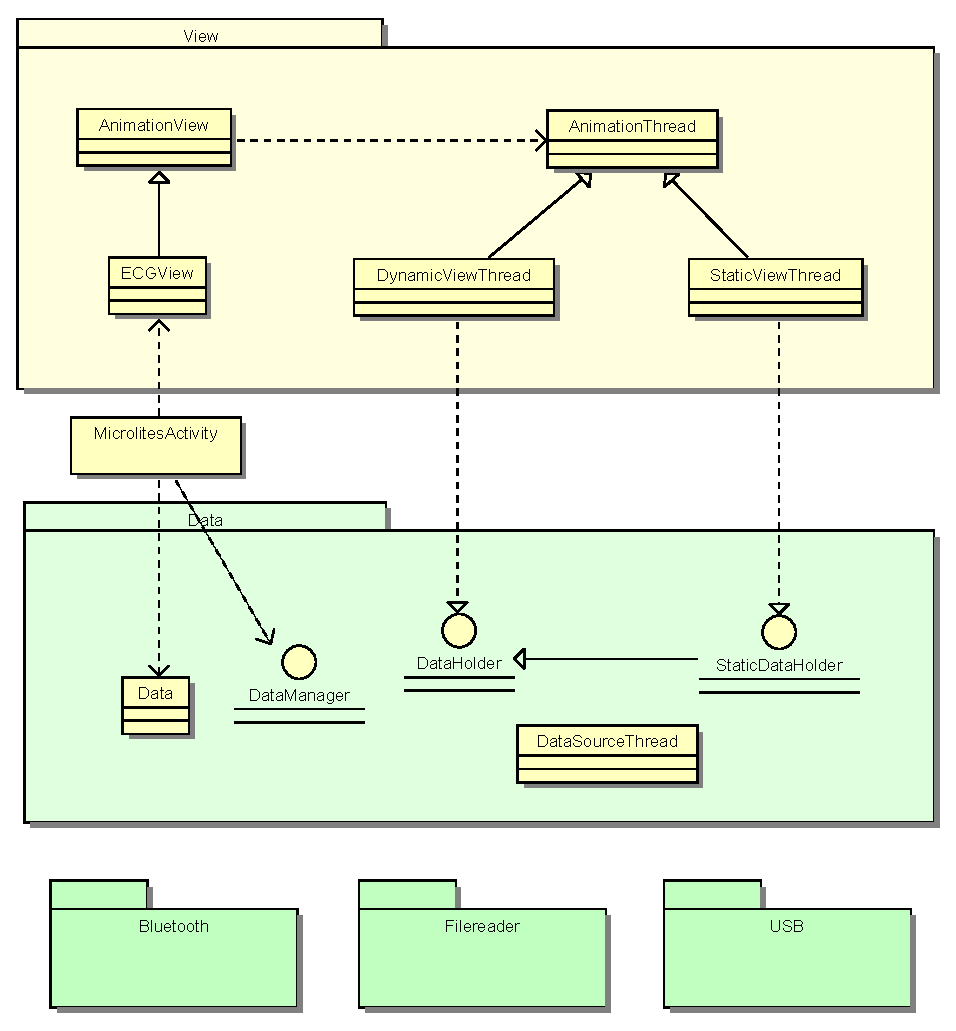
\includegraphics[scale=0.75]{mlts-arch-main}
		\centering
		\caption{Architecture overview}
		\label{fig:arch-global}
		\end{figure}

		At the core level the main Activity, the View package and the Data package are present, as well as three packages (Bluetooth, Filereader, USB) which will be dealt with later. These components provide the basic elements which compose the model over which actual functionality is built, and are to be seen as the tools available for the overlaying software layer which is addressed next.\\

		The main Activity of the application assumes the role of the central coordinator and is responsible for creation and management of area specific managers, application level data and handling of the aforementioned user interfaces stack. It is also responsible, as the application's entry point, of the presentation and behaviour management of the main application menu which gives access to actual functionality, delegating in the specific managers.\\
		
		Of all those tasks, the most important are the initialization and eventual finalization of data visualization flows in collaboration with the appropiate area specific manager. Throughout the process, mainly controlled by the activity, components required for the visualization process are initialized, delegating area specific tasks to the manager. Eventually, the manager assumes the control of the application flow, leaving the activity as a dispatcher of input events.\\

		% Model: Core, domain specific components that require realization in order to work.
		% Model involves: a Manager, a DataSource and a DataHolder (as well as a DataParser) and, if visualization is required, the ECGView and a ViewThread derivate.
		% The model needs to be realized for it to work, the Activity is just an engine running an instance of the model.
		% "It follows a factory pattern, but the factory is the Activity."

		These managers are part of the so-called, in the project terminology, a model; and the activity can be portrayed as the model manager. Conceptually a model is a set of software entities which live in the application and handle the data flow from a given data source towards a data holder, including or not, the visualization of such data. A model contains a Manager which is the entity responsible of the handling of the rest of the model entities. Please note that this model scheme is  specific to the domain of the project and is not a general one\todo{Remove this note? Leave this note?}.

		\begin{figure}[h]
		\includegraphics[scale=0.75]{mlts-arch-model}
		\centering
		\caption{Data-flow model realization}
		\label{fig:arch-model}
		\end{figure}

		This conceptual model \todo{Rename model to FlowModel?} scheme is provided by a subset of the classes and interfaces shown in \autoref{fig:arch-global}. For actual functionality building a realization of the model is to be developed, giving actual meaning to the scheme. In the scope of the project four model realizations have been implemented and will be detailed later.\\

		A model realization is composed of implementations of the following elements from the core level exposed before: 1) a Manager, which handles user interaction and required preparations; 2) a DataSource that manages raw data obtention from the actual source, and processing and sending of such data to a 3) DataHolder, which stores and handles the data in any required way and, if data visualization is required 4) an implementation of a view thread.\\

		More detailed approaches to all the concepts exposed in this introduction are built throughout the following subsections.

		\subsection{View Package}
		\begin{comment}
		Realtime rendering required a special, non full common functionality (slide, scroll, ...) providing View derivate: SurfaceView. It provides a bitmap surface where you can draw whatever you want. Derived into AnimationView with employment of AnimationThread for obtaning a good old while(!finished) \{update(); render();\} loop.
		That structure derivates into ECGView which is a domain specific specialization of AnimationVeiw and Dynamic- and StaticViewThread. The later two implement behaviour expected of Dynamic and Static data visualization respectively (more on this on the Data Package)
		Programming style in this area closer to C than to an OOP language in order to maximize performance. (Talk about intolerable initial performance caused by extreme number of new each step and too much relaying on GarbageCollector?)
		\end{comment}

		The set of classes encompassed in the View package (see \autoref{fig:arch-global}) provides both a base rendering architecture in an update-render loop style not initally present in the Android framework and the specialization of such architecture for the specific project domain, i.e. plotting of the electrocardiogram wave and its relevant points.\\

		Regarding rendering Android provides a set of common employed visual elements. These implementations try to simplify the developer's work by giving customizable solutions to common scenarios, such as rendering a list of elements or a drop-down selection object, in a visually pleasing way. All this elements are part of the hierarchy of Android's View class, and implement a composite pattern for rich menu-building.

		The soft real-time rendering imposed by the project restrictions requires a specific View \todo{reference to View in andev?} class derivate: the SurfaceView. This kind of View provides a bitmap surface where pixel-level rendering is allowed. A set of rendering tools is also provided by Android. The architecture developed on top of that view extends the SurfaceView to an AnimationView and delegates the rendering to an AnimationThread. This last entity is the one providing the update-render loop employed for the real-time rendering. The drawback of employing a SurfaceView as the base is that such element doesn't provide common employed functionality as scrolling or zooming.\\

		The actual, domain specific rendering functionality providing threads are implemented employing the aforementioned layer as a base. The precise entities are DynamicViewThread and StaticViewThread, and are referred in this document as implementations of the view thread, even if such class does not exist in the project. This two classes implement the required behaviour for dynamic and static data visualization respectively, and obtain the data to be shown from a data source entity. Such entity is dealt with in the following section. The reason for different entities to exist for static and dynamic rendering is also detailed there.\\

		\subsection{Data Management Package}
		\begin{comment}
		Data class acting as a centralized data storage. Provides app-level synchronization too.
		Different models for static and dynamic data management.
		Dynamic: manages its own data and implements replacemente and discard politics, data is provided by single units. This is so because of the way the data is received and then parsed in real-time.
		Static: obtains a reference to the data location, which is where the actual data manipulation is done. This way huge ammounts of data transfering is avoided (read file can contain lots of megabytes of data which can't be passed at once to the holder). First try was passing the whole array of samples but that was unassumable in real-time.
		DataSourceThread is a receiver by concept, but concrete implementations might require actual communication, that is, data reception \emph{and} data sending. As a developer facility, any DataSourceThread must provide an implementation of a method for writing data into the actual raw data source, expected to act in a similar manner to the one the DataSourceThread does in the inside.
		\end{comment}
		
		This package contains data storage and handling related entities. Differentiation between two types of data managed by the application depending on their purpose is mandatory. On one hand is the application level data, which is specific or non-specific information shared by the whole application. On the other hand is the data received from a source that must be visually presented to the user or stored for later visualization. Providing software tools allowing the modelling that data flow is the key task of this package.\\

		The class Data acts as a centralized application level data storage. It is a singleton and is accesible by every entity in the system. It also provides syncronization methods for correct inter-thread communication.\\

		The rest of the entities of the Data package are employed in the aforementioned model scheme, and specify the expected behaviour of each element involved in a data flow. As indicated before, specialization of this entities is required for the realization of the model.\\

		%\begin{wrapfigure}{l}{0.35\textwidth}
		\begin{figure}[h]
		\begin{center}
	    	\includegraphics[width=0.20\textwidth]{mlts-ent-datamanager}
  		\end{center}
  		\caption{DataManager interface}
		\end{figure}
		%\end{wrapfigure}


		DataManager is the interface to be implemented by the model controller. It is responsible for the configuring, starting and halting the data flow provided by its controlled entities. It also participates in the process of initialization of the visualization \todo{Link to this process} of a data flow by communicating a DataHolder with the respective DataSourceThread.\\

		A DataSourceThread is a thread which provides data to other entities in the system, generally to a DataHolder. It is a specialization of Thread with functionality to start and stop the flow of data. This data is usually received from an external entity, such as a USB device or a file, and concrete implementations  might require an actual communication between the two, forcing the DataSourceThread to send data to the other end of the connection. Because of that, any specialization of this class must also listen to petitions of writing to its data provider when available.\\

		%\begin{wrapfigure}{l}{0.35\textwidth}
		\begin{figure}[h]
		\begin{center}
	    	\includegraphics[width=0.3\textwidth]{mlts-ent-datasource}
  		\end{center}
  		\caption{DataSourceThread class}
		\end{figure}
		%\end{wrapfigure}

		The processing of raw data sent by the data providers to the DataSourceThreads is expected to be done in the latter, so the data transfered throughout the application is of a processed nature. To this end the DataParser entity is available\todo{Reference DataParser}.\\

		The expected receiver of the data sent by a DataSourceThread is a DataHolder. This interface provides domain-specific data handling abstract methods and definitions. An implementation of a DataHolder must handle the reception of ECG wave samples, delineation points, synchronization points and heart-beat-rate values.\\

		%\begin{wrapfigure}{l}{0.35\textwidth}
		\begin{figure}[h]
		\begin{center}
	    	\includegraphics[width=0.20\textwidth]{mlts-ent-dataholder}
  		\end{center}
  		\caption{DataHolder interface}
		\end{figure}
		%\end{wrapfigure}

		The actual way in which that data is employed depends on the concretion of the interface, and might or might not involve visual representation. When visual representation is required, the view thread implementation should also implement the DataHolder interface.\\

		%Dynamic: manages its own data and implements replacemente and discard politics, data is provided by single units. This is so because of the way the data is received and then parsed in real-time.
		%Static: obtains a reference to the data location, which is where the actual data manipulation is done. This way huge ammounts of data transfering is avoided (read file can contain lots of megabytes of data which can't be passed at once to the holder). First try was passing the whole array of samples but that was unassumable in real-time.

		There are two different specifications for the data holders: DataHolder and StaticDataHolder. This is so because of the two modes of operation\todo{Is it clear that there are two modes of operation?} of the application. One is real-time data visualization and the other is log file visualization. The former is called dynamic visualization and the latter static visualization, and the behaviour of their DataHolders is not the same.\\

		Dynamic visualization represents data received in realtime by the DataSourceThread. The DataSourceThread obtains the data from an external entity, processes it and sends it to the DataHolder. This data usually arrives in groups of variable size, and is provided to the DataHolder in single units once processed. In this scenario the DataHolder is the view thread, and handles data however considers optimal. In the implementations developed in this project a fixed amount of data is held and older information is replaced by the new one as it arrives.\\

		Static visualization, on the other hand, involves reading a file, usually megabyte sized. The receiving of big quantities of data in single units by the data holder, as would occur if  the original DataSource specification was employed, could lead to severe slow-downs and application performance would be affected. To avoid such issues, the StaticDataHolder specification is developed.\\

		A StaticDataHolder does not actually hold the data: it delegates that task to its DataSourceThread. The data source will provide the StaticDataHolder with a reference to the actual data. This way big amounts of data transferring is avoided. The inheritance relation between DataHolder and StaticDataHolder is imposed by the architecture, which require a DataHolder to be passed to a DataSourceThread.\\

		\subsection{Utilities Package}
		\begin{comment}
		Contains application level reusable components as two different DataParsers (one for realtime, on for static data which doesn't store what it reads). Also contains the Viewport entity employed as a container of the view parameters. An unused color picker is there (not mention!)
		\end{comment}
		This package contains reusable components providing very specific functionality so they are considered utilities: RealTimeDataParser, StaticDataParser and Viewport.\\

		A data parser is the entity responsible of the processing of the raw data obtained by a DataSource into the domain specific data that the application manages. There are two implementations, one for real-time data reception, RealTimeDataParser, and the other for static data reading, i.e. a log file. The real-time data parser is also responsible of storing the received raw data to a log file.\\

		A data parser is intended to be contained in a DataSourceThread. It receives the bytes of raw data and, upon successful identification of a valid data element, notifies the corresponding DataHolder entity of the arrival. In a theoric, performance-independant model, this behaviour would be incorrect: the data parser would leave the processed data \emph{in} the DataSourceThread, which would then make the transfer of information to the data holder. This kind of implementation is not valid with the soft realtime requirements of the project, as the data source - data parser - data source - data holder flow would be a severe bottle-neck.\\

		The Viewport entity is a container for the visualization area settings. It represents the window in which the data plotting is done, and holds information about size and position of it. It also contains data about the horizontal and vertical scale of the rendering and handles modification of all these parameters. It is employed by the view thread hierarchy.
		
		\subsection{Data Flow Model Realizations}

		Having explained the data flow model scheme and the core level architectural elements employed in its construction, model realizations implemented are detailed next. For each realization, the concretion of each model element will be exposed including particular details of such implementation.

		\subsubsection{Bluetooth Model}
			The Bluetooth \todo{Bluetooth (TM)?} model is a real-time visualization targeted data flow where the actual data provider is a Bluetooth node. As visualization is an objective, this model realization employs a DataManager, a DataSource, a DataHolder and a DynamicViewThread; the latter two being implemented in the same entity. An overview of the realization is shown in \autoref{fig:arch-bt}.\\

			\begin{figure}[h]
			\centering
		    	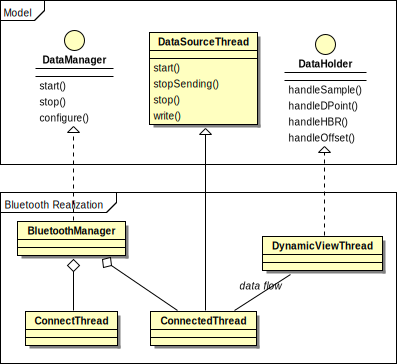
\includegraphics{mlts-arch-bt}
	  		\caption{Bluetooth Model Realization}
			\label{fig:arch-bt}
			\end{figure}

			The specialization of the DataManager is the BluetoothManager. It prompts the user for the device to connect to and handles connection by employing two threads: ConnectThread and ConnectedThread. After discovering the available nodes, it locates the node indicated by the user and launches the ConnectionThread.\\

			This ConnectThread is the thread which actually manages the connection by obtaining its endpoints in the form of a socket. If successful, passes the socket to the manager and finishes its execution. The manager then launches the ConnectedThread, which receives the socket and data flow starts. The reason for employing a thread for establishing the connection is to avoid blocking the application while connecting.\\

			ConnectedThread is the DataSourceThread implementation and contains an entity of DataParser. It receives data sent by the Bluetooth device through the socket, parses it and notifies the DataHolder implementation, which is the DynamicViewThread. The DataParser in DataSourceThread is a RealTimeDataParser and stores the data in a log file while processing.

		\subsubsection{File Reader Model}
			This model realization implements visual representation of ECG data stored in a log file. It is a static view model, in which the user controls what section of the temporal log is shown on-screen, an thus employs an StaticViewThread instead of a dynamic one.\\

			\begin{figure}[h]
			\centering
		    	\includegraphics{mlts-arch-log}
	  		\caption{File Reader Model Realization}
			\label{fig:arch-log}
			\end{figure}
		
			The manager in the file reader model is the FileManager class. It presents available log files to the user, handles the seleccion of one, instantiates the file reading thread and connects this with the view thread. When the user finalizes the visualization of the selected log, the FileManager returns to the log selection menu instead of going directly to the main menu. This is an example of the versatility of the aforementioned view stack scheme, which lets specific managers present as many menus to the user as necessary.\\

			FileDataSourceThread is the thread that reads the chosen file and processes its data. It implements both the DataSource and the DataHolder interfaces, so it acts as the emitter and the receiver of the processed data. The view thread obtains a reference to this same data, thus avoiding big amounts of data transferring in the static view model as explained before. This is an example of the flexibility sought by the architecture design.\\

			The FileDataSourceThread, thus, manages data reading, storage and manipulation. The data is read from files with the aid of this package's FileConverter entity. This files can be of big size, so they should not be fully loaded onto memory. A partial load is mandatory in such cases, and the next chunk of data is to be read when the ``visualization window'' approaches. All this management is done by the FileDataSourceThread.\\

			When the view is controlled by the user, i.e. horizontal scroll, the event is passed directly into this thread from the StaticViewThread. FileDataSourceThread then updates the portion of the data to be shown. The updated information is consulted by the view thread in the next rendering step. That way, were further file reading required, it could be done in a transparent-to-view manner.\\

			Data processing is done employing an instance of StaticDataParser in the FileDataSourceThread.\\

			The FileConverter entity provides functionality to transform a given file to a Stream, ArrayList or array of bytes, the latter being the expected input format for the available data parsers.

		\subsubsection{USB Model}
			The USB model manages data reception from an USB device and eventual visual representation for the user. It is a real-time data flow, and thus employs a dynamic view thread. An overview of the model is shown in \autoref{fig:arch-usb}.\\

			\begin{figure}[h]
			\centering
		    	\includegraphics{mlts-arch-usb}
	  		\caption{USB Model Realization}
			\label{fig:arch-usb}
			\end{figure}

			DeviceManager is the realization of the model's Manager. This entity handles connected USB devices enumeration and selection by the user. If only one device is available, connection is directly stablished with it. Differing from the Bluetooth realization implementation, the actual connection to the device is handled by the DeviceManager in a blocking manner. It is so because USB connection resolution takes very little time and the delay is virtually imperceptible for the user.\\

			Once the connection is stablished, the DeviceManager launches a UsbComThread. This thread is the specialization of DataSourceThread and obtains the raw data from the USB device, processes it employing an instance of DynamicDataParser and sends the results to the view thread. This is a DynamicViewThread entity.

		\todo{USER INTERFACES! New subsection with diagrams and all? as an Appendix?}

		\begin{comment}
		\subsection{More things (which I don't know where to include}
			
			\texttt{(These with sequence diagrams and all)}
			Explanation of the visualization initialization procedure, as well as the finalization one.
			Example of a full data flow (e.g. bluetooth)
		\end{comment}

	\section{Implementation Details}

		\begin{comment}
			Potential iterations
			It1. Bluetooth + Architecture prototype
			It2. USB + Log
			It3. Architecture rewriting
			It4. Adding it all and finishing

			For iteration description:
				+ objectives
				+ objectives description
					realization, done?
				+ Use Cases realized
				+ expected and spent time
				+ extra objectives
				+ prologue to next iteration

			Describe risk statuses updates in each iteration?
		\end{comment}

		% Intro
		In this section a detailed description of the development is presented. The evolution of the application architecture and functionality; design, architectural and implementation decisions and explanations of the circumstances in which they were made, as well as the development of the project schedule are exposed in chronological order.\\

		The section is arranged following the five iterations of the project, developing each one by presenting the target objectives and expected deadlines for the iteration, detailing application evolution with emphasis on use case realization and risk suppressing achievements and demonstrating the state of the project as assessed on the reviewing meeting conducted at the end of the iteration.

		% Scheduling
		\subsection{Project Scheduling}
			
			Before diving into the description of the development process an overview of the project schedule % and the reasons for it to be as open as it is
			is mandatory.\\

			As was mentioned in the previous sections, an agile software development methodology has been applied to the project, even if artifacts from more ordered and structured methodologies have been employed to avoid losing focus on the critical aspects of the development.\\
	
			Software development project being dependant on parallel-conducted hardware research, project assets, both personal and development resources, being shared with the hardware research having the former higher priority, and team's lack of formation regarding Android development are some of the factors which lead to the adoption of such a mixed methodology. As they have been already exposed in previous sections, they won't be detailed here.\\ %Consult [X][Y][Z]... for details

			In such an scenario, a fully developed, eight month covering schedule was unfeasible, at least with the imposed time restrictions which didn't allow much time to be spent on planning. The decision was then made to plan only the earlier project iterations, assuring critical functionality identified from use case development to be implemented as soon as possible as well as higher threat involving risk suppression to be realized.\\

			Actual software project development begun October 15, 2011, being the final deadline set on June 15, 2012. That deadline could not be pushed any further, so an estimated deadline was set on May 31, 2012, leaving half a month for further work or recovering from delays, and seven and a half months of development time.\\
		
			Time was needed for the hardware research to start providing results, and no work could be done in the meantime on related application parts. Considering also that even in the most optimistic scenarios no actual work with the 802.15.4 USB receiver couldn't be done until mid February [link to hw planning or something], the schedule had to assume that the first four months of software development would need to cover the implementation of most of the features, leaving the rest of the development time for implementing hardware-related requirements, which couldn't actually be scheduled until hardware research was evaluated.\\

			The adopted schedule dealt with the aforementioned facts by proposing five iterations, from October 15 to May 30, complying with the fifteen days reserved for contingencies. The first three iterations had a duration of two months, the third one a single month, and the remaining one was fifteen days long.\\

			Having the previously developed iOS application as starting point, and being achieving at least the same feature list of that a critical target of the project, the first two iterations were planned so as to realize \textbf{UC1} and \textbf{UC3} which captured requisites expressing such feature list.\\

			The next iterations were just scrapped as no accurate estimation could be done on the state of the project by those dates. Thus, the third iteration was planned to cover the implementation of the remaining features, namely, communication with the 802.15.4 receiver device, the fourth one reserved for polishing the application and the fifth one left for testing and validation. The fourth iteration was to shrink if objectives were achieved quickly to leave more time for validation.\\

			The scheduled distribution of work for each iteration is as follows:\\

			\begin{tabular}{| c | l | l |} % | l | para el hw
				\hline
				It & Dates & Activity \\ \hline
				1 & Oct 15 - Dec 15 & Application base and Bluetooth module\\ \hline
				2 & Dec 15 - Feb 15 & Log module and initial USB module\\ \hline
				3 & Feb 15 - Apr 15 & Final USB implementation \\ \hline
				4 & Apr 15 - May 15 & Polishing \\ \hline
				5 & May 15 - May 30 & Validation \\ \hline
				- & May 30 - Jun 15 & Reserved \\
				\hline
			\end{tabular}\\\\

			Which can be seen as the following expected use case realization dates:\\

			\begin{tabular}{| c | l | l |} % | l | para el hw
				\hline
				It & Dates & Realized Use Case \\ \hline
				1 & Oct 15 - Dec 15 & UC1, UC4 (first version)\\ \hline
				2 & Dec 15 - Feb 15 & UC3, UC2 (first version)\\ \hline
				3 & Feb 15 - Apr 15 & UC2 (final) \\ \hline
				4 & Apr 15 - May 15 & UC4 (final) \\ \hline
				5 & May 15 - May 30 & Validation \\ \hline
				- & May 30 - Jun 15 & Reserved \\
				\hline
			\end{tabular}\\\\

			Throughout the development, as expected, this schedule had to be adapted as the hardware research advanced to assess the arise of difficulties and subsequent changes to its planning. Instead of providing a fixed snapshot of the altered schedule at the end of the project, a detailed description of each iteration is presented next, including modifications to the planning and the motivation for making them.

		\subsection{Iteration 1}

			The main objectives for this first iteration were
			\begin{itemize} 
				\item the instruction of the team on Android development, 
				\item the lay out of an initial version of the application architecture and
				\item the implementation of the Bluetooth receiver module.
			\end{itemize}

			The alloted time for the iteration was of two monts, from October 15 to December 15. During this period the hardware research didn't require much resources [link to hw], so in practical terms the full team was employed in the software project.\\

			In order to minimize risk AR1[quote?link?], the instruction of the team on Android development becomes the key objective for the iteration. Development starts with the implementation of the designed base architecture for the application, so it serves as a powerful learning resource. The notion of that implementation as disposable is not abandoned throughout iteration time and it is always considered as a prototype to evolve or be substituted by a more refined version once team's knowledge of Android increases.\\

			Having the basic architectural framework developed, implementation of the Bluetooth receiver module begins. Special care is put both on design and implementation, as this functionality has to be ready as soon as posible, and little time will be available for reimplementation further in the development.\\

			Testing of both architecture and Bluetooth module is conducted during the whole iteration, specially in the final weeks, so by the end of the iteration Bluetooth module is validated and expected to be stable until the scheduled architectural redesign.\\

			As the Android formation phase takes less time than expected and hardware research doesn't allow advancing into next iteration at the time iteration objectives are achieved, an extra implementation effort is put to begin implementation of UC4. Adjust View Parameters.\\

			In the review meeting for the iteration the following conclusions are obtained:
			\begin{itemize}
				\item Basic architecture implementation is done.
				\item Android is confirmed to be a very comfortable development environment even if non-standard functionality is not that easily achieved. Instruction is planned to continue.
				\item Realization of UC1-\emph{View data from Bluetooth} is finished. Related user interface is not final, but it is functional, and is to be updated on further iterations.
				\item Realization of UC4-\emph{Adjust view parameters} is done in relation to Bluetooth visualization. As remaining modules are developed, further work is to be done in this field.
			\end{itemize}

			\begin{comment}
			Results and adaptation of pre-planned it2
			Risk evolution!?
			\end{comment}
			
		\subsection{Iteration 2}

			The main objectives for the second iteration are
			\begin{itemize} 
				\item the development of the USB communication module and
				\item the implementation of the Log visualization module.
			\end{itemize}

			The hardware reserarch having provided successful results regarding the initial prototypes of the USB accessory, the scheduled USB module implementation for this iteration is mantained, but delayed until further testing can be done in the hardware area.
			In that scenario this iteration begins by the addressing of the implementation of the log visualization module. \todo{This sentence sounds odd, to be fair/kind.}\\

			Module design and implementation are to change little in following iterations to allow the scheduled architecture rewriting to be realized and trying to minimize the possibility of risk PR1. This situation and the fact that a lot of resources are required in the hardware area makes the consecution of this objective fill most part of the iteration time.\\

			Full expected functionality is implemented, including the remaining features from UC4-Adjust view parameters, but validation testing indicates low performance in log visualization caused by big memory requirements. Effort needs to be put into the other iteration objective, so log visualization is halted at this point, scheduling the development of required optimizations for the next iteration.\\

			Having the USB accessory prototype in an usable state, development of the USB communication module begins. At this point the USB accessory could only operate assuming the role of host in the connection, so the disposability of the module is acknowledged. Nevertheless, this implementation is a must if the project goals are to be achieved, as it serves as first-hand instruction regarding USB development in Android. Moreover, if the hardware project is unable to produce an USB slave accessory, with the developed module the project would not have fully failed. Eventually this development has proven being key for the first tests with the actual target hardware platform.\\

			During the implementation of the USB communication module the log writing is improved, so, except for the aforementioned performance optimizations, the log part of the application is finished.\\

			With the basic interface, disposable architecture and fully functional data flow modules, full application functionality is implemented by the end of the iteration, and in the review meeting the following conclusions are obtained:
			\begin{itemize}
				\item Full functionality has been implemented in the application and the product of this iteration is, as expected, the first prototype of the application.
				\item Realization of UC2-\emph{View data from USB Receiver} is realized until hardware research advances. Current implementation can act as the actual version of the use case realization if hardware research is not fulfilled.
				\item Realization of UC4-\emph{Adjust view parameters} is now finished. All required view controls are implemented.
				\item Risk PR1-\emph{Application functionality inferior to that featured by existing iOS application} is marked as surpassed, as key functionality is implemented.
				\item Risk MR1-\emph{Mobile device unsuitable for target functionality} is identified to require further monitorization and is unfolded into risks AR2 and AR3.
				\item Risk AR2-\emph{Android providing subpar performance when handling required data} is confirmed to occur and is to be solved in the next iteration.
			\end{itemize}

			\begin{comment}
			Log writing improved.
			USB module done as USB device, valid for arduino and first msp tests
			Log reading implemented, scrolling and such. Tests results indicate low performance, huge memory requirements.
			With the basic interface, first Prototype with (except usb host == 802.15.4) full functionality implemented. That nice and all. Shown to masters and feedback applied.
			On time ?
			
			Took a loong break here for hardware development
			% Here ends electroiltes
			\end{comment}

		\subsection{Iteration 3}
			% This is microlites
			\begin{comment}
			This is the first just-drafted iteration. Starting from the fully functional prototype, architectural and performance fixes were mandatory. Also, given the positive state of the hw research scheduling was done for the rest of the iterations.

			The main objectives for this third iteration are
			\begin{itemize} 
				\todo{Remove leading ``the's'' to improve readability?}
				\item the redesign of the application architecture, 
				\item the achievement of required performance in data management and
				\item the scheduling of the rest of the project time.
			\end{itemize}

			~(Scheduling seems strange as an objective)~

			Architecture redesigned targeting easy adaptation and versatility inside the scope of the application. Redesigned visualization initialization flow.
			Performance increased significantly and memory usage reduced THROUGHOUTLY in realtime view.
			Fixes in modules according to new architecture.
			Talk about scheduling??
			\end{comment}

			This is the first just-drafted iteration of the original scheduling. Taking the prototype obtained in the previous iteration, architectural redesign and performance optimizations are mandatory. Performance optimizations are  identified to be required in two areas: data management and data rendering. Only data management related optimizations are addressed in this iteration.\\

			Iteration objectives are as follow:
			\begin{itemize} 
				\item redesign of the application architecture, 
				\item achievement of required performance on data management, and
				\item scheduling of the rest of the project time.
			\end{itemize}

			The main lack of the basic architecture of the protoype is that it was implemented to serve as a quick prototyping base for the data flow modules. The instruction and knowledge about the platform and the way of operation obtained in the previous iterations are applied in the new architecture design.\\

			This design is done targeting easy inclusion of new data flow modules allowing them to employ their own user interfaces, while providing core level software entities for building those modules. This process produces the architecture as exposed in \autoref{sec:sw-arch}.\\

			A detailed analysis is conducted on the data management related operations in the application, identifying the ubiquitous application of the object oriented model proposed by Java added to the subpar efficiency of the Garbage Collector \todo{Reference something? Could be added a screenshot from that Eclipse performance analysis tool?} as the main cause of performance loss. The alteration of the programming paradigm and the employment of as basic software entities as possible, substituting classes\todo{Perhaps ``avoiding continuous object instantiation'' better?} used to, e.g. contain the four parameters of a wave delineation point, by more basic structures, like the same four numbers stored independently, proved to be the most effective methods of avoiding low performance.\\

			Following such lines of operation, performance regarding data management is utterly improved on spite of a less developer-friendly programming environment. During this process the data flow modules (Bluetooth, USB and Log Viewer) are also tweaked.\\

			The positive results obtained both in the software and hardware areas allow a solid review of the project schedule. The decision is made to keep the division of the remaining project time in two iterations, leaving the last, fifteen days period for unforseen difficulties. Of the two iterations, the first is to be devoted to implementation of the USB host communication as hardware project estimates completion of a first prototype halfway the iteration; and the second, and last, iteration is planned to be employed in final testing and validation of the application against hardware prototype.\\

			The following conclusions are obtained from this iteration's reviewing meeting:
			\begin{itemize}
				\item The architecture of the application is finished and validated.
				\item User interface is yet to be final and is to be addressed at the following iteration.
				\item Identified solutions for performance issues are to be applied in the rendering area.
				\item Risk AR1-\emph{Lack of instruction on Android development delays workflow} is marked as surpassed as the team feels comfortable enough with Android development.
				\item Risk AR3-\emph{Android rendering capabilities unable to handle required data} probability is increased to Moderate and is to be addressed in the next iteration.
				\item Risk HR2-\emph{802.15.4 receiver device unfeasibe} probability is reduced to Low as hardware research is providing positive results.
			\end{itemize}

		\subsection{Iteration 4}
			\begin{comment}
			Final implementation iteration. Final performance increasing fixes and user interface implementation, as well as user-friendliness globally increased.

			USB Host here!

			The main objectives for this third iteration were
			\begin{itemize} 
				\item the implementation of USB host communication,
				\item the achievement of required performance in rendering and, 
				\item the implementation of user-friendly interfaces.
			\end{itemize}

			This ends the implementation phase, user-friendlyness could be better but what gives. 
			Performance left 50-50 because it was already ok (30fps not 60fps).
			One iteration left, devoted to testing.
			\end{comment}

			This iteration is scheduled to be the last implementation iteration, and it's objectives are:
			\begin{itemize} 
				\item the implementation of USB host communication,
				\item the achievement of required performance in rendering and, 
				\item the implementation of actual user interfaces.
			\end{itemize}

			The USB slave accessory prototype is produced on time by the hardware project, and implementation of the actual USB communication assuming the Android device the host role is done in very short time, leaving room for consecution of the rest of the iteration objectives and following validation.\\

			Employment of the identified working solutions for performance issues in the rendering area doesn't provide the expected results, and further research is required. The bottle-neck in the rendering process is indentified to be the context change required by the rendering tools provided by Android. Meticulous research on Android developer resources provides no other solution than minimizing the number of calls to the rendering methods each step. Emphasis is put to the realization of this task, but to no avail.\\

			The problem is the big amount of data required to be drawn each rendering step. A mechanism is developed to minimize the number of lines drawn by joining similar valued wave points, and the performance is improved, but not at the desired level. Nevertheless further work in this area is postponed as the achieved performance lies in the range required by the non-functional requirements of the project.\\

			Implementation of the actual user interfaces to be employed in the application is addressed next. The design of these has been done throughout the last two iterations. The implementation process takes more time than expected as	Android user interface framework is quite specific, and requires adequation to certain rules that have to be studied beforehand.\\

			The remaining time of the iteration is devoted to testing and validation of the application, which has reached a near final state. Conclussions from the review meeting follow:
			\begin{itemize}
				\item The Android application is finished and pending validation with the actual USB receiver device.
				\item The application's user interface is in a final state, but were changes required they could be easily implemented as the UI is isolated from the data flow part.
				\item Performance regarding rendering is not optimal, but it is in the range defined by the requisites.
				\item Until validation can begin, the full team can be employed in the hardware project.
				\item Risk HR2-\emph{802.15.4 receiver device unfeasible} is marked as surpassed as the viability of the receiver has been proved by the hardware research.
			\end{itemize}

		\subsection{Final Validation}
			The final effort in this software project extends over the allotted time for both the fifth iteration and the reserved final period. It is fully devoted to testing and validation of both the application and the receiver device. Even if the initial schedule assigned only the fifth iteration to this process, delays on the hardware project \todo{reference hw chapter} force the elongation of the testing phase.

			The objectives for this period are:
			\begin{itemize}
				\item exhaustive testing of the Android application,
				\item validation of the application, the receiver and the delineator node acting as a whole, and
				\item the obtention of the final version of the system by implementing the required amendments identified by the testing procedure.
			\end{itemize}

			Software related testing is conducted throughout all this final step causing minor fixes to be done to the application. No relevant software related issues arise during the testing or the validation phases.\\

			Risk HR1-\emph{802.15.4 receiver device delayed} occurrence is the cause of the elongation of the validation iteration, but has no actual effect on the software project. Even when the receiver is completed \todo{Maybe in a prototype stage, still unknown at Jun, 8} the risk tracking is continued until validation concludes, were hardware complications to arise during the process.\\

			The final, review meeting conclusions are as follow:
			\begin{itemize}
				\item Risk HR1 is marked as surpassed.
				\item The Android application is successfully validated and, thus, completed.
			\end{itemize}
			
	\section{Closure}

		The software development part of the project has been able to produce the required Android application, with all planned functionality implemented and including user friendly interfaces. It is a rather general purpose application inside of the domain to which it is restricted, and at it's final state it would need some specialization in order to be actually useful. This is so because the requisite analysis process wasn't developed focusing an immediate professional employment of the application, but a replacement for that of the EPFL project which inspired this one. \\

		Anyhow, during the architecture design and subsequent implementation phases great emphasis is put for the application to provide the tools to act as a framework over which more specific ECG montoring application development can be realized.\todo{Something from Marian feature list here?} An interesting example of this is that, at the current state, the application implements visualization of data received from an USB device. In this project, the USB device has been the 802.15.4 USB receiver, but any other device capable of encoding the data in the expected way is valid as well.\\

		Long story short, the software development finished providing successful results in form of a general purpose ECG monitoring application for Android devices which can serve as the base for more specific developments, which was exactly the target objective for the software project.

	\chapter{Results}
\label{cha:results}

	\section{Final state}
	\label{sec:end-state}
	
		% Describes the fulfillment of this project.

		\todo{Describe battery usage, size requirements actual data}
		% The production of a fully functional, low cost and low sized ECG monitoring system which employs an Android device as the user interface, and it's USB 802.15.4 receiver is completed.\\

		The production of the fully functional, low energy requiring, low sized ECG monitoring system employing an Android device as the user interface and 802.15.4 as the wireless data transferring protocol has been achieved. The system provides all the required functionality: real-time ECG wave data visualization both from 802.15.4 and Bluetooth nodes and storing of the received data in log files for afterwards visualization of these, as well as visualization parameters configuration. The system is, then, a more energy efficient and accessible version of the one produced by the Complutense University of Madrid and the École Polytechnique Fédérale de Lausanne, which is the primary objective of the project.\\

		This achievement is made thanks to the successful outcome of both the hardware research and the software development processes in which the project has been divided. Each of them requiring the employment of specific methodologies and techniques, but being, as they were, highly dependent one on the other only complicated the prediction of the outcome of them both. Thanks to the flexible scheduling conducted for each one, which considered the potential eventualities to arise in the other and focused in allowing rescheduling when necessary, this uncertainty has been correctly managed, leading to the current, successfully finalized state of the project.\\
		
		% HW: The goal of an external 802.15.4 receiver device is fulfilled. Employing it the system is able to render ECG data emitted by a delineator node. Bluetooth is also available, as well as log saving and further reading.\\
		% No olvidar hablar de modificaciones al shimmer!
		Regarding the hardware research part, the main goal pursued was the production of the 802.15.4 USB receiver device for Android systems. This device has successfully evolved from the early stages of development where a prototyping board was employed to a custom developed printed circuit board, which, if has not been produced, is completely designed and validated\todo{Not yet, but soon}.\\

		% Concrete results: X x Y x Z sized device consuming W1 watts of power (actual data, please) which compared to Bluetooth consumption (W2 watts, ...) is pretty low cost, all of this powered by the Android device, and the receiver being plug and play no installation procedure is required.\\
		The prototype board's \todo{Substitute these for the PCB ones if available}dimensions are 7.25 x 6.35 x 3.5 cm, and it requires 3.3V for correct operation, being usable with at least 3.0V. Its USB capability allows for it to be connected to any HID compliant system, and has been successfully employed as an 802.15.4 receiver both in Android devices and Windows based personal computers.\\

		In respect of the Android application, the software development project has produced an Android application providing all required functionality, namely visualization of ECG data from Bluetooth and USB nodes, log saving and reading, and view controlling capabilities, designed and implemented in a robust, expandable manner. Moreover, the application provides a domain-specific framework for the inclusion of new data sources (like Wi-Fi or Near Field Connection) or different source data specifications.\\

		The application presents simple, easy to use user interfaces and very specific functionality, which added to the following of Android proposed application design best-practices smooth the learning curve and allow out of the box usage of the software part of the system. Due to the expansion capabilities of the system, new user interfaces or dialogs can also be added with ease.\\
	
	\section{Potential additions and expansions}
	\label{sec:end-further}
		\begin{comment}
		Potential additions are to target the software frontend application. The developed Android application is a (domain specific) general purpose monitoring frontend that should provide a solid framework for further developments.\\

		Professional multipatient monitoring could come in two flavours:\\

		Visual-less multipatient monitoring in which a computer receives data from a variable number of wireless delineation nodes, e.g. employing the 802.15.4 receiver, storing it and acting as a server, or directly sending the log files to the actual server. The Android device would then download the log from the server and the own frontend application developed in the scope of this project could be used as the visualization device.\\

		The other option is simultaneous multipatient monitorization in an Android device. The monitorization application on the device would allow switching between patient ECG wave visualization while logging all received data, which could then be uploaded to a server.\\

		(Both of these expansions could find an employment in acutal medical environment.)


		More improvements can include the implementation of more detailed log navigation functionality, including information about the actual recording time and searching of specific time moments.
		Inclusion of event data into the log (like body weakness sensation or feeling of dizziness) could also be useful.
		(This two are for personal monitorization and inhome healthcare)\\

		Message sending when certain events occur (low or high hbr or arrythmia detection), text message, email, even a phone call could help constant monitorization requiring people. GPS information could be included in the message for quick localization of the affected person by the healthcare personal.

		% Comentar también como trabajo futuro los requisitos que plantea Marian
		\end{comment}

		Although every initially planned objective has been fulfilled, in addition to several of them which
		were added during the development, there is still room for improvements and features which were
		not considered or left out of scope, since the developed application is not considered as a specific
		product itself, but a framework for further developments. These improvements can be classified according 
		to the period planned for their implementation:

		\begin{itemize}
			\item \textbf{Short-term:} the following features specifically target personal use. Considering
				the user is to monitor his/her own vital signs, the next additions are thought to be useful:

				\begin{itemize}
					\item \emph{Event Tagging}\\
						Assuming the user is feeling funny or pain, it may be quite interesting for him/her
						to be able to annotate such an event with later revision purposes, either by
						him/herself or medical staff. Furthermore, the capability of marking down one peculiar
						result about the ECG delineation can also be useful.\\

						In this way, making use of the tactile interface the Android tablet features, this
						activity can be done by simply touching the relevant event or result. Next, the moment
						which that points refers is logged and a comment may be added to the annotation.\\

					\item \emph{Temporal Meta-Data}\\
						In the same conditions described in the previous item, it is possible that the user
						had felt a particular sensation in a certain moment, yet he/she was unable to mark it.
						Moreover, maybe the annotation was done and it is required to directly jump to that
						certain time.\\

						In order to ease these tasks, time-related data is to be added so that a precise
						moment of the monitoring can be directly found. In this way, the user can input
						the desired date so that the application shows what was happening at that moment.
						In addition, markers from previous annotations would also appear for quickly accessing
						to relevant events.\\

					\item \emph{Voice Commands}\\
						Due to the particular health condition of the user, or just because he/she is busy,
						direct interaction with the monitoring Android device is likely to be impossible. If
						situations like these are to happen, letting users interact with the system through
						their own voice may ease the aforementioned tasks.\\

						Fortunately, Android provides speech recognition support throughout its specific API,
						so this feature could be added without developing the whole voice recognition framework.\\

					\item \emph{Automatic Warnings}\\
						Regarding the user's health condition or unavailability again, automatic message sending
						with ECG data in case of relevant happenings were detected would mean a seamless way to
						warn the user, relatives or qualified staff if needed. In the same direction, multiple
						alternatives would be presented such as emails with GPS location attachments or direct
						automatic voice calls to complement this feature.

				\end{itemize}

				All these features come from a potential project proposed by an specific individual, which, 
				being affected of a certain cardiovascular disease and considering the goals and results of 
				this specific project, has shown interest in further specialization of the developed system for
				particular needs. This private enterprise is yet to be started, but the inception phase has already
				begun, and is seeking funding. The team of the current project is offering consulting on the
				viability of the requirements of the project, and testing has been conducted of the already
				available system with the interested individual.\\

			\item \textbf{Long-term:} this features are mainly ideas which would grant the system with much 
				richer capabilities and new potential, though it would require of a greater amount of time
				along with specific planning and dedication.\\

				On the one hand, the application can be focused towards professional multipatient monitoring,
				which could be developed in at least two alternative ways:

				\begin{itemize}
					\item Since the developed 802.15.4 USB receiver is also compatible with HID-compliant
						devices, particularly computers, multipatient monitoring could be uploaded to a
						devoted server from a variable number of wireless delineaton nodes, omitting the 
						displaying service the Android application provides. Once the data is uploaded,
						the Android device could connect with the mentioned server and download the information
						right from the developed application. Then, the Android tablet would act as usual
						as frontend of the monitoring process, displaying the downloaded data.

					\item Taking into account the relatively big display a tablet device provides, this
						multipatient monitoring paradigm could be directly implemented into the Android 
						device by extending the application's functionality. Among this new functionalities
						there would be switching between ECG wave visualizations of different patients,
						simultaneous logging and server uploading as well.
				\end{itemize}

				On the other hand, regarding self-monitoring, the system can be adapted to be applied to 
				specific domains which impose additional time or resource restrictions.
				Specifically the director of the Embedded Systems Laboratory at the EPFL, where the delineator 
				node employed in this project was produced in the aforementioned collaboration with the UCM, 
				has shown interest in the application of the low power requirements of system in a specific project
				the EPFL is collaborating with: Solar Impulse \cite{solarflight}.\\

				This particular project tries to achieve a flight around the world employing no fuel, just the
				energy collected from the sun. The airplane used in the project allows only for the pilot to be
				in the cockpit throughout the flight, and, thus, he/she is required to be constantly monitorized.
				Among others, ECG monitorization is required, at is, at the time, being provided by the EPFL and
				UCM monitoring project with the already exposed battery implications of the employment of 
				Bluetooth as the wireless technology.\\

				Considering that the space in the cockpit is very reduced, and the amount of wires, sensors and
				other instruments that are present, any operation is to be done with special care and only when
				absolutely needed. Concretely, the swapping of a battery-exhausted delineator node for another,
				fully-charged one, to allow the recharging of the first, is a complex procedure as the body
				sensor network wires have to be unplugged from one node and plugged into the other. Moreover,
				while this procedure is being performed ECG monitorization is interrupted.\\

				Reducing the battery consumption of the delineator node is then, a must, and can be achieved by
				the employment of 802.15.4 as the wireless communication protocol. Because of that, the results
				obtained in this project can of great use to the Solar Impulse project.\\
	
		\end{itemize}
	
	\section{Findings}
	\label{sec:end-findings}

		Development:
		
		Employment of Android for this real-time thingamagigs is not the best thing ever as, even if the devices have high computational power, the restrictions imposed by the operating system hardens the task quite a lot. In that scenario a custom display device would allow finer, prettier visualization of the data, BUT of course the benefits of employing Android like 1. it's already developed duh 2. simplicity of development of visually rich apps and, specially, 3. high availability of the devices which reduces the amount of devices carried, compensate for every drawback it may have. So, asuming some limitations in the display applications (which already can eventually or will be able to be overcome) the selection of Android as a platform has been awesomely great.

		Regarding the process of a project such as this that spawn various subprojects with different characteristics and highly related one on the other, the employment of a flexible schedule, a detailed risk management procedure and focusing a lot on the current objective and it's deadline is critical for a successful outcome.

		Results:

		Ideas: importance of monitorization systems for cardiovascular diseases affected people. Great potential of development in this area. Low cost, low sized, user focused designed, an thus, comfortable application system development is a ineherntly good goal, as are of great help for CVD affected people.

		In this line, 802.15.4 as a low energy requiring wireless protocol significantly reduce the need of monitorization interruption due to battery recharging procedures, which seems like a small thing but is extra nice for minimizing the impact in the life style of the affected people. Also, employment of Android instead of iOS allows things like letting the application work in background while doing other things, shall not be interrupted by an incoming call and such. Also seem like small things but hell if you have to cope with them in day after day.

		Interesting: Marian is interested in the project for personal monitorization, David Atienza (EPFL's ESL \& UCM) is highly interested in the lower energy costs this project has achieved. Also, Solar Flight.


	% Anexos
	\begin{appendices}
		\renewcommand{\setthesection}{\Alph{section}}	% Numeramos con letras
		\appendix
		\appendixpage
		\chapter{Budget Analysis}
\label{ch:budget}

	Throughout this appendix the project budget analysis is conducted, by detailed specification of both time and resource cost.
	The project division in atomic tasks and the scheduling of these.
	
	\section{Project tasks and sheduling}

		\begin{figure}[h]
			\centering
		    	\includegraphics[width=\textwidth]{gantt-l}
			\label{fig:gantL}
		\end{figure}
		\begin{figure}[h]
			\centering
		    	\includegraphics[width=\textwidth]{gantt-r}
			\label{fig:gantR}
		\end{figure}

		\begin{tabular}{| c | p{7cm} | l | l |} % | l | para el hw
		\hline
T1.1.1 & Acquire a suitable Android device prototyping environment & 15/10/2011 & 16/11/2011\\ \hline
T1.1.2 & Manage correct communication between Android and a prototype device & 17/11/2011 & 11/12/2011\\ \hline
T1.1.3 & Develop an application emulating desired behaviour & 12/12/2011 & 19/12/2011\\ \hline
H1 & Arduino for Android USB device Communication & 19/12/2011 & 19/12/2011\\ \hline
T1.2.1 & Supply MSP430 with USB protocol application functionality & 20/12/2011 & 04/01/2012\\ \hline
T1.2.2 & Research Android USB protocol related functionality & 05/01/2012 & 19/02/2012\\ \hline
T1.2.3 & Make Android OS recognize MSP430 when plugged	 & 20/02/2012 & 22/02/2012\\ \hline
T1.2.4 & Manage communication between Android and MSP430 via USB & 23/02/2012 & 07/03/2012\\ \hline
H2 & MSP430 for Android USB Host Comunication & 08/03/2012 & 08/03/2012\\ \hline
T1.3.1 & Check the proper working of FreeRTOS with the new microcontroller & 09/03/2012 & 13/03/2012\\ \hline
T1.3.2 & Validate the feasibility of the usage of USB API along with FreeRTOS in MSP430 & 14/03/2012 & 23/03/2012\\ \hline
T1.3.3 & Correctly integrate USB API into FreeRTOS & 24/03/2012 & 31/03/2012\\ 
\hline
\end{tabular}\\\\

\begin{tabular}{| c | p{6cm} | l | l |} % | l | para el hw
\hline
T1.3.4 & Manage USB data sending in FreeRTOS & 31/03/2012 & 02/04/2012\\ \hline
H3 & USB in FreeRTOS & 02/04/2012 & 02/04/2012\\ \hline
T1.4.1 & Validate current implementation of 802.15.4 in FreeRTOS in MSP430 testing board & 03/04/2012 & 18/04/2012\\ \hline
T1.4.2 & Manage connection to the CC2420 radio module to target MSP430 device & 19/04/2012 & 21/04/2012\\ \hline
T1.4.3 & Port implementation of 802.15.4 to target MSP430 device & 22/04/2012 & 28/04/2012\\ \hline
T1.4.4 & Prepare such implementation for actual usage & 28/04/2012 & 09/05/2012\\ \hline
H4 & 802.15.4 in FreeRTOS & 09/05/2012 & 09/05/2012\\ \hline
t1.5.1 & Assess conflict-free coexistence of current implementation of both USB and 802.15.4 modules in MSP430 & 10/05/2012 & 16/05/2012\\ \hline
T1.5.2 & Manage sending data received from 802.15.4 via USB & 17/05/2012 & 25/05/2012\\ \hline
H5 & 802.15.4 \& USB coexistence under FreeRTOS & 25/05/2012 & 25/05/2012\\ \hline
T1.6.1 & Exhaustive analysis of the reference board & 10/05/2012 & 21/05/2012\\ \hline
T1.6.2 & Capture of the board schematic & 21/05/2012 & 14/06/2012\\ \hline
T1.6.3 & Design and routing of the actual PCB & 15/06/2012 & 21/06/2012\\ \hline
H6 & MSP430 based device design & 21/06/2012 & 21/06/2012\\ \hline
T1.7.1 & Final validation of final aplications with prototyping hardware & 26/05/2012 & 16/06/2012\\ \hline
T1.7.2 & Final validation of final aplications with final hardware & Not performed & Not performed\\ \hline
H7 & Final Validation and Release Candidate Version Development & 15/06/2012 & 15/06/2012\\ \hline
IT1 & Completed UC1 & 15/10/2011 & 15/12/2011\\ \hline
   T2.1.1 & Instruction of the team on Android development & 16/10/2011 & 07/11/2011\\ \hline
   T2.1.2 & Lay out of an initial version of the application architecture & 06/11/2011 & 19/11/2011\\ 
\hline
\end{tabular}\\\\

\begin{tabular}{| c | p{6cm} | l | l |} % | l | para el hw
\hline
   T2.1.3 & Implementation of the Bluetooth receiver module & 14/11/2011 & 03/12/2011\\ \hline
IT2 & Completed UC4, UC3 & 15/12/2011 & 04/02/2012\\ \hline
   T2.2.1 & Development of the USB communication module & 05/01/2012 & 20/01/2012\\ \hline
   T2.2.2 & Implementation of the Log visualization module & 15/12/2011 & 28/01/2012\\ \hline
IT3 & Completed Redesign	15/02/2012 & 15/04/2012\\ \hline
   T2.3.1 & Redesign of the application architecture & 16/02/2012 & 12/03/2012\\ \hline
   T2.3.2 & Achievement of required performance on data management & 13/03/2012 & 28/03/2012\\ \hline
   T2.3.3 & Scheduling of the rest of the project time & 28/03/2012 & 05/04/2012\\ \hline
IT4 & Completed UC2 & 12/04/2012 & 11/05/2012\\ \hline
   T2.4.1 & Implementation of USB host communication & 16/04/2012 & 26/04/2012\\ \hline
   T2.4.2 & Achievement of required performance in rendering & 22/04/2012 & 07/05/2012\\ \hline
   T2.4.3 & Implementation of actual user interfaces & 28/04/2012 & 11/05/2012\\ \hline
IT5 & Final Validation & 15/05/2012 & 22/06/2012\\ \hline
   T2.5.1 & Exhaustive testing of the Android application & 15/05/2012 & 22/06/2012\\ \hline
   T2.5.2 & Validation of the application, the receiver and the delineator node acting as a whole & 26/05/2012 & 22/06/2012\\ \hline
   T2.5.3 & Obtention of the final version of the system by implementing the required amendments identified by the testing procedure. & 21/05/2012 & 17/06/2012\\
\hline
\end{tabular}\\\\


\section{Asset cost}

	A partir de la planificación anterior, que es la real del proyecto, y considerando que hubo en total cerca de dos meses de vacaciones, podemos considerar que este proyecto tiene una duración de 7 meses con 3 personas trabajando a media jornada. Tipicamente el salario de un ingeniero trabajando en este campo sería de unos 35 euros la hora. Por lo que el coste de un ingeniero durante 7 meses a media jornada sería 35euros/hora * 4 horas/dia * 22 dias/mes * 7 meses = 21560\\

	Este coste, unido al de los productos que habría habido que adquirir si no hubiera habido nada en el lugar donde se realizase el proyecto nos dan el coste total del proyecto:\\

\begin{tabular}{| p{5cm} |l | l | l |} 
\hline
   Name & Number& Price per unit & Total price\\ \hline
   Motorola Xoom - Wifi & 1 & 399 & 399\\ \hline
   Google ADK & 1 & 70,8 & 70,8\\ \hline
   Exp430F5438 + MSP430F5438A & 1 & 117,89 & 117,89\\ \hline
   TS430PZ100USB + 2xMSP430F6638 & 1 & 60 & 60\\ \hline
   CC2420 & 1 & 4,00 & 4,00\\ \hline
   Prototype & 1 & 38,60 & 38,60\\ \hline
   Final product & 1 & 42,229 & 42,229\\ \hline
   Enginer & 3 & 21560 & 64680\\ \hline
   Total & & & 65392,13\\ \hline
\hline
\end{tabular}\\\\


\chapter{Product Cost}
\label{ch:cost}

	El coste de fabricar un dispositivo de manera individual, que es lo que se ha hecho durante el proyecto es el siguiente:\\

\begin{tabular}{| c |l | l | l | l |} 
	\hline
		Name & Reference & Number & Price per unit & Total price\\ \hline
		SMT & 1022311 & 2 & 1,96 & 3,92\\ \hline
		Resistor & 1738981 & 2 & 0,062 & 0,124\\ \hline
		LED & 1699413 & 1 & 0,28 & 0,28\\ \hline
		Capacitor & 1833863 & 6 & 0,03 & 0,18\\ \hline
		Capacitor & 1740650 & 2 & 0,154 & 0,308\\ \hline
		Capacitor & 499110 & 2 & 0,114 & 0,228\\ \hline
		Resistor & 1469918 & 1 & 0,038 & 0,038\\ \hline
		Capacitor & 1833865 & 2 & 0,144 & 0,288\\ \hline
		Diode & 1469389 & 3 & 0,099 & 0,297\\ \hline
	   	Capacitor & 1833803 & 1 & 0,085 & 0,085\\ \hline
 		Capacitor & 1327699 & 1 & 0,36 & 0,36 \\ \hline
  		Resistor & 1500615 & 4 & 0,028 & 0,112\\ \hline
	 	Capacitor & 644183 & 1 & 0,27 & 0,27 \\ \hline
	 	Capacitor & 1740632 & 1 & 0,062 & 0,062\\ \hline
	 	MSP430F6638 & 2070274 & 1 & 18,49 & 18,49\\ \hline
	 	Capacitor & 1833888 & 1 & 0,163 & 0,163\\ \hline
	 	Capacitor & 499160 & 2 & 0,122 & 0,244\\ \hline
	 	ESD protection & 1269406 & 1 & 0,63 & 0,63\\ \hline
	 	Microcrystal & 1539364 & 1 & 2,19 & 2,19\\ \hline
	 	Capacitor & 1658880 & 2 & 1,98 & 3,96\\ \hline
	 	%MGRID & 1756749 & 8 & 0,057 & 0,456\\ \hline NO VAN EN EL PRODUCTO
	 	%Header & 7472285 & 1 & 1,34 & 1,34\\ \hline NO VAN EN EL PRODUCTO
	 	%Milligrid & 511031 & 1 & 0,163 & 0,163\\ \hline NO VAN EN EL PRODUCTO
	 	Radio & From TI & 1 & 4,00 & 4,00\\ \hline
		Production & & 1 & 6,00 & 6,00\\ \hline
	 	Total &  &  &  & 42,229\\ \hline
	\hline
\end{tabular}\\\\

	Como todo producto hardware, el precio por unidad suele ser muy elevado pero a partir de cantidades de producción algo más levadas se reduce sustancialmente, para 
	ilustrarlo este sería el coste de 10000 unidades:\\

\begin{tabular}{| c |l | l | l | l |} 
	\hline
		Name & Reference & Number & Price per unit & Total price\\ \hline
		SMT & 1022311 & 20000 & 1,65 & 33000\\ \hline
		Resistor & 1738981 & 20000 & 0,017 & 340\\ \hline
		LED & 1699413 & 10000 & 0,156 & 1560\\ \hline
		Capacitor & 1833863 & 60000 & 0,005 & 300\\ \hline
		Capacitor & 1740650 & 20000 & 0,032 & 640\\ \hline
		Capacitor & 499110 & 20000 & 0,024 & 240\\ \hline
		Resistor & 1469918 & 10000 & 0,01 & 100\\ \hline
		Capacitor & 1833865 & 20000 & 0,024  & 480\\ \hline
		Diode & 1469389 & 30000 & 0,053 & 1590\\ \hline
	   	Capacitor & 1833803 & 10000 & 0,025 & 250\\ \hline
 		Capacitor & 1327699 & 10000 & 0,063 & 630 \\ \hline
  		Resistor & 1500615 & 40000 & 0,021 & 840\\ \hline
	 	Capacitor & 644183 & 10000 & 0,159 & 1590 \\ \hline
	 	Capacitor & 1740632 & 10000 & 0,012  & 120\\ \hline
	 	MSP430F6638 & 2070274 & 10000 & 13,07 & 130700\\ \hline
	 	Capacitor & 1833888 & 10000 & 0,026  & 260\\ \hline
	 	Capacitor & 499160 & 20000 & 0,041  & 820\\ \hline
	 	ESD protection & 1269406 & 10000 & 0,42  & 4200\\ \hline
	 	Microcrystal & 1539364 & 10000 & 1,40 & 14000\\ \hline
	 	Capacitor & 1658880 & 20000 & 1,03  & 20600\\ \hline
	 	%MGRID & 1756749 & 80000 & 0,043  & 0,456\\ \hline NO VAN EN EL PRODUCTO
	 	%Header & 7472285 & 10000 & 1,34 & 1,34\\ \hline NO VAN EN EL PRODUCTO
	 	%Milligrid & 511031 & 10000 & 0,163 & 0,163\\ \hline NO VAN EN EL PRODUCTO
	 	Radio & From TI & 10000 & 4,00 & 40000\\ \hline
		Base board &  & 1 & 100 & 100\\ \hline
		Production &  & 10000 & 0.05 & 500\\ \hline
	 	Total &  &  &  & 252860\\ \hline
	 	Total per unit &  &  &  & 25,286\\ \hline
	\hline
\end{tabular}\\\\












	\end{appendices}

	% Bibliografía
	\fancyhf{}
	\fancyfoot[RO,LE]{\thepage}
	\renewcommand{\headrulewidth}{0.0pt}
	\renewcommand{\footrulewidth}{0.0pt}
	\begin{thebibliography}
{widest-label}

%\bibitem{journal:itjq12002}{\it Hyper-Threading Technology},
%Intel Technology Journal,
%Volume 06 Issue 01,
%Published February 14 2002,
%ISSN: 1535766X

%\bibitem{HaNO97} {\it A single-chip multiprocessor},
%L. Hammand, B. A. Nayfeh, \& K. Olukotum,
%IEEE Computer, 30(9):79-85,Sep. 1997.

%\bibitem{libro:lkd}{\it Linux Kernel Development},
%Rovert Love,
%Ed. Sams Publishing, 2004,
%ISBN: 0-672-32512-8

%\bibitem{paper:sched2681}{\it Understanding the Linux 2.6.8.1 CPU Scheduler},\newline
%Josh Aas (\href{mailto:josh@trancesoftware.com}{josh@trancesoftware.com})\newline
%\copyright 2005 Silicon Graphics, Inc. (SGI)\newline
%17th February 2005\newline
%\href{http://josh.trancesoftware.com/linux/}{http://josh.trancesoftware.com/linux/}

\end{thebibliography}


\end{document}
